% ============================================================
%  Macro Country Analysis – Oral Presentation
%  Denmark · Norway · Sweden
%  15 min total | 5 min per person
% ============================================================
\documentclass[aspectratio=169,11pt]{beamer}

\usepackage{tikz}
\usepackage{booktabs}
\usepackage{graphicx}
\usepackage{xcolor}
\usepackage{array}
\usepackage{colortbl}

% ---------- colour palette ----------
\definecolor{navydark}{HTML}{1A2742}
\definecolor{dkred}{HTML}{C60C30}
\definecolor{norred}{HTML}{EF2B2D}
\definecolor{sweblue}{HTML}{006AA7}
\definecolor{lightgray}{HTML}{F2F2F2}

% ---------- theme ----------
\usetheme{Madrid}
\usecolortheme[named=navydark]{structure}
\setbeamercolor{frametitle}{bg=navydark,fg=white}
\setbeamercolor{title}{bg=navydark,fg=white}
\setbeamercolor{block title}{bg=navydark!80,fg=white}
\setbeamertemplate{navigation symbols}{}
\setbeamerfont{frametitle}{size=\large,series=\bfseries}
\setbeamerfont{framesubtitle}{size=\small}

% ---------- section-separator macro ----------
\newcommand{\sectionslide}[3]{%
  \begin{frame}[plain]
    \begin{tikzpicture}[remember picture,overlay]
      \fill[#1] (current page.south west) rectangle (current page.north east);
      \node[white,font=\Huge\bfseries] at (current page.center) {#2};
      \node[white,font=\large,yshift=-1.2cm] at (current page.center) {#3};
    \end{tikzpicture}
  \end{frame}
}

% ---------- helper: compact stat row ----------
\newcolumntype{L}{>{\raggedright\arraybackslash}p{3.2cm}}
\newcolumntype{R}{>{\raggedleft\arraybackslash}p{1.5cm}}

% ============================================================
\title[Macro Country Analysis]{Macroeconomic Country Analysis}
\subtitle{Denmark · Norway · Sweden}
\author{Group Presentation}
\date{Spring 2026}
% ============================================================

\begin{document}

% ── TITLE SLIDE ─────────────────────────────────────────────
\begin{frame}[plain]
  \begin{tikzpicture}[remember picture,overlay]
    \fill[navydark] (current page.south west) rectangle (current page.north east);
    \node[white,font=\LARGE\bfseries,yshift=1.0cm]
          at (current page.center) {Macroeconomic Country Analysis};
    \node[white,font=\large,yshift=0.1cm]
          at (current page.center) {Denmark \quad|\quad Norway \quad|\quad Sweden};
    \node[white,font=\normalsize,yshift=-0.8cm]
          at (current page.center) {Penn World Table 11.00 · FRED · Solow Growth Model};
    \node[white,font=\small,yshift=-1.8cm]
          at (current page.center) {Spring 2026};
    % flag colour stripes at bottom
    \fill[dkred]   ([yshift=0.45cm]current page.south west)
                   rectangle ([yshift=0.15cm]current page.south east);
    \fill[norred]  ([yshift=0.15cm]current page.south west)
                   rectangle ([yshift=-0.15cm]current page.south east);
    \fill[sweblue] ([yshift=-0.15cm]current page.south west)
                   rectangle ([yshift=-0.45cm]current page.south east);
  \end{tikzpicture}
\end{frame}

% ============================================================
%  PART 1 – DENMARK
% ============================================================
\sectionslide{dkred}{Denmark}{\textcolor{white!70!dkred}{Economic Data \& Solow Model}}

% ── DK 1: GDP per capita ────────────────────────────────────
\begin{frame}{Denmark – GDP per Capita}
  \framesubtitle{Trend growth $\approx1.0\%$ p.a. since 2000 (1995 Q1 – 2024 Q4)}
  \begin{columns}[T]
    \begin{column}{0.62\textwidth}
      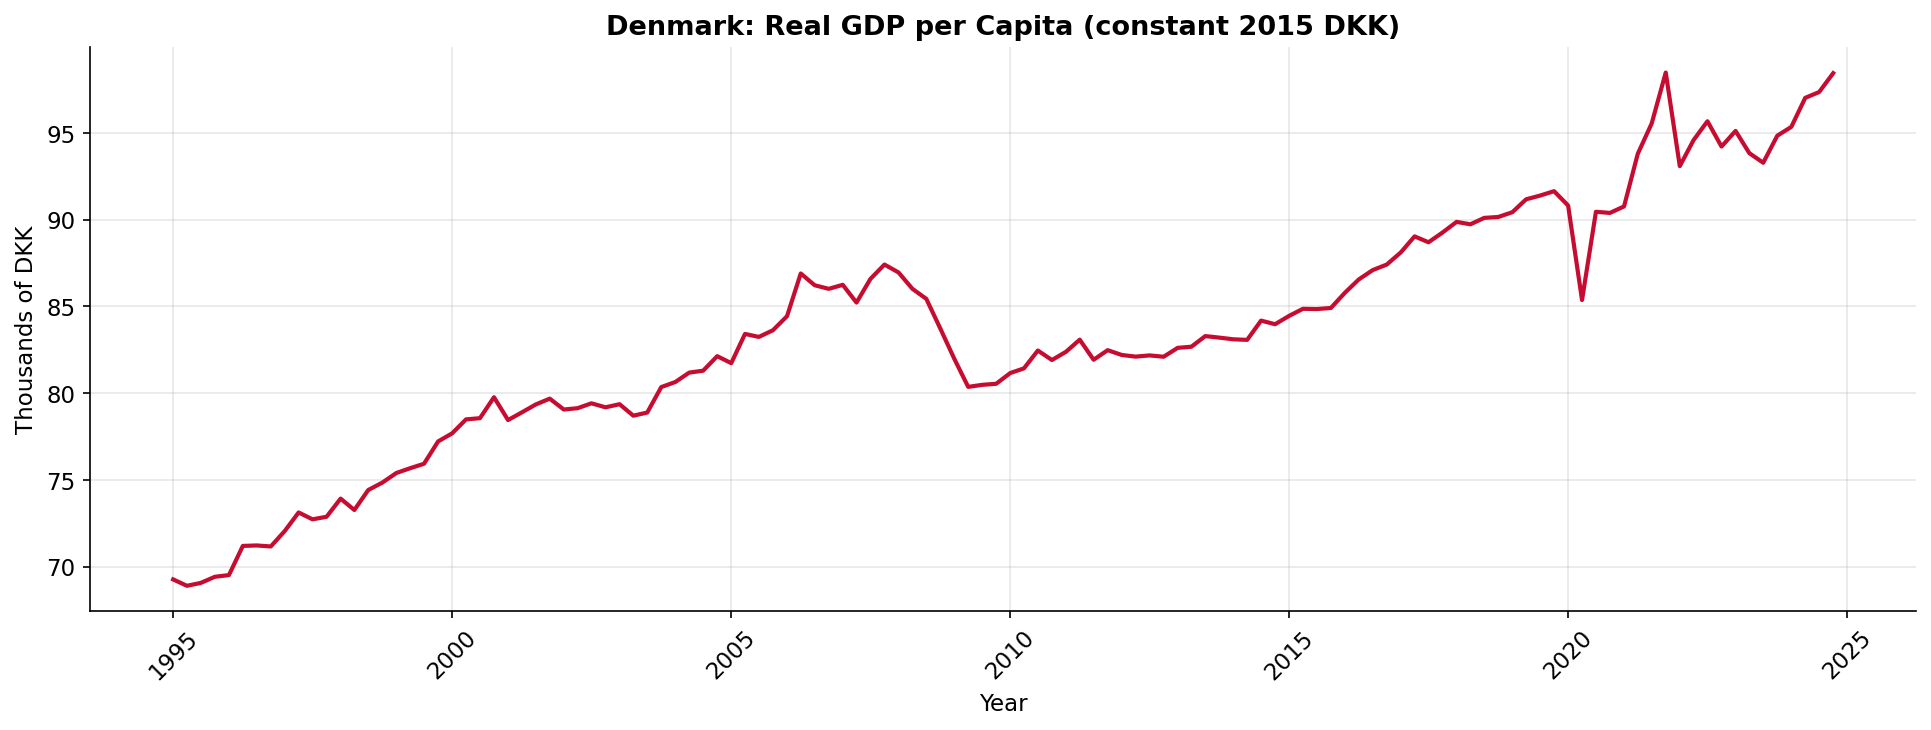
\includegraphics[width=\linewidth]{Denmark/denmark_gdp_pc_level.png}
    \end{column}
    \begin{column}{0.35\textwidth}
      \vspace{0.3cm}
      \small
      \begin{tabular}{@{}Lr@{}}
        \toprule
        \textbf{Indicator} & \textbf{Value} \\
        \midrule
        Sample & 1995–2024 \\
        Trend growth & $\approx1.0\%$ p.a. \\
        GFC drop & $\approx-7\%$ \\
        COVID drop & $\approx-5\%$ \\
        \bottomrule
      \end{tabular}
      \vspace{0.5cm}
      \begin{itemize}\setlength\itemsep{3pt}
        \item Sustained convergence to high-income level
        \item Clear 2008–09 recession trough
        \item Rapid post-COVID recovery
      \end{itemize}
    \end{column}
  \end{columns}
\end{frame}

% ── DK 2: Business Cycles ───────────────────────────────────
\begin{frame}{Denmark – Business Cycles}
  \framesubtitle{HP-filtered output gap ($\lambda=1600$) · Unemployment \& Inflation}
  \begin{columns}[T]
    \begin{column}{0.48\textwidth}
      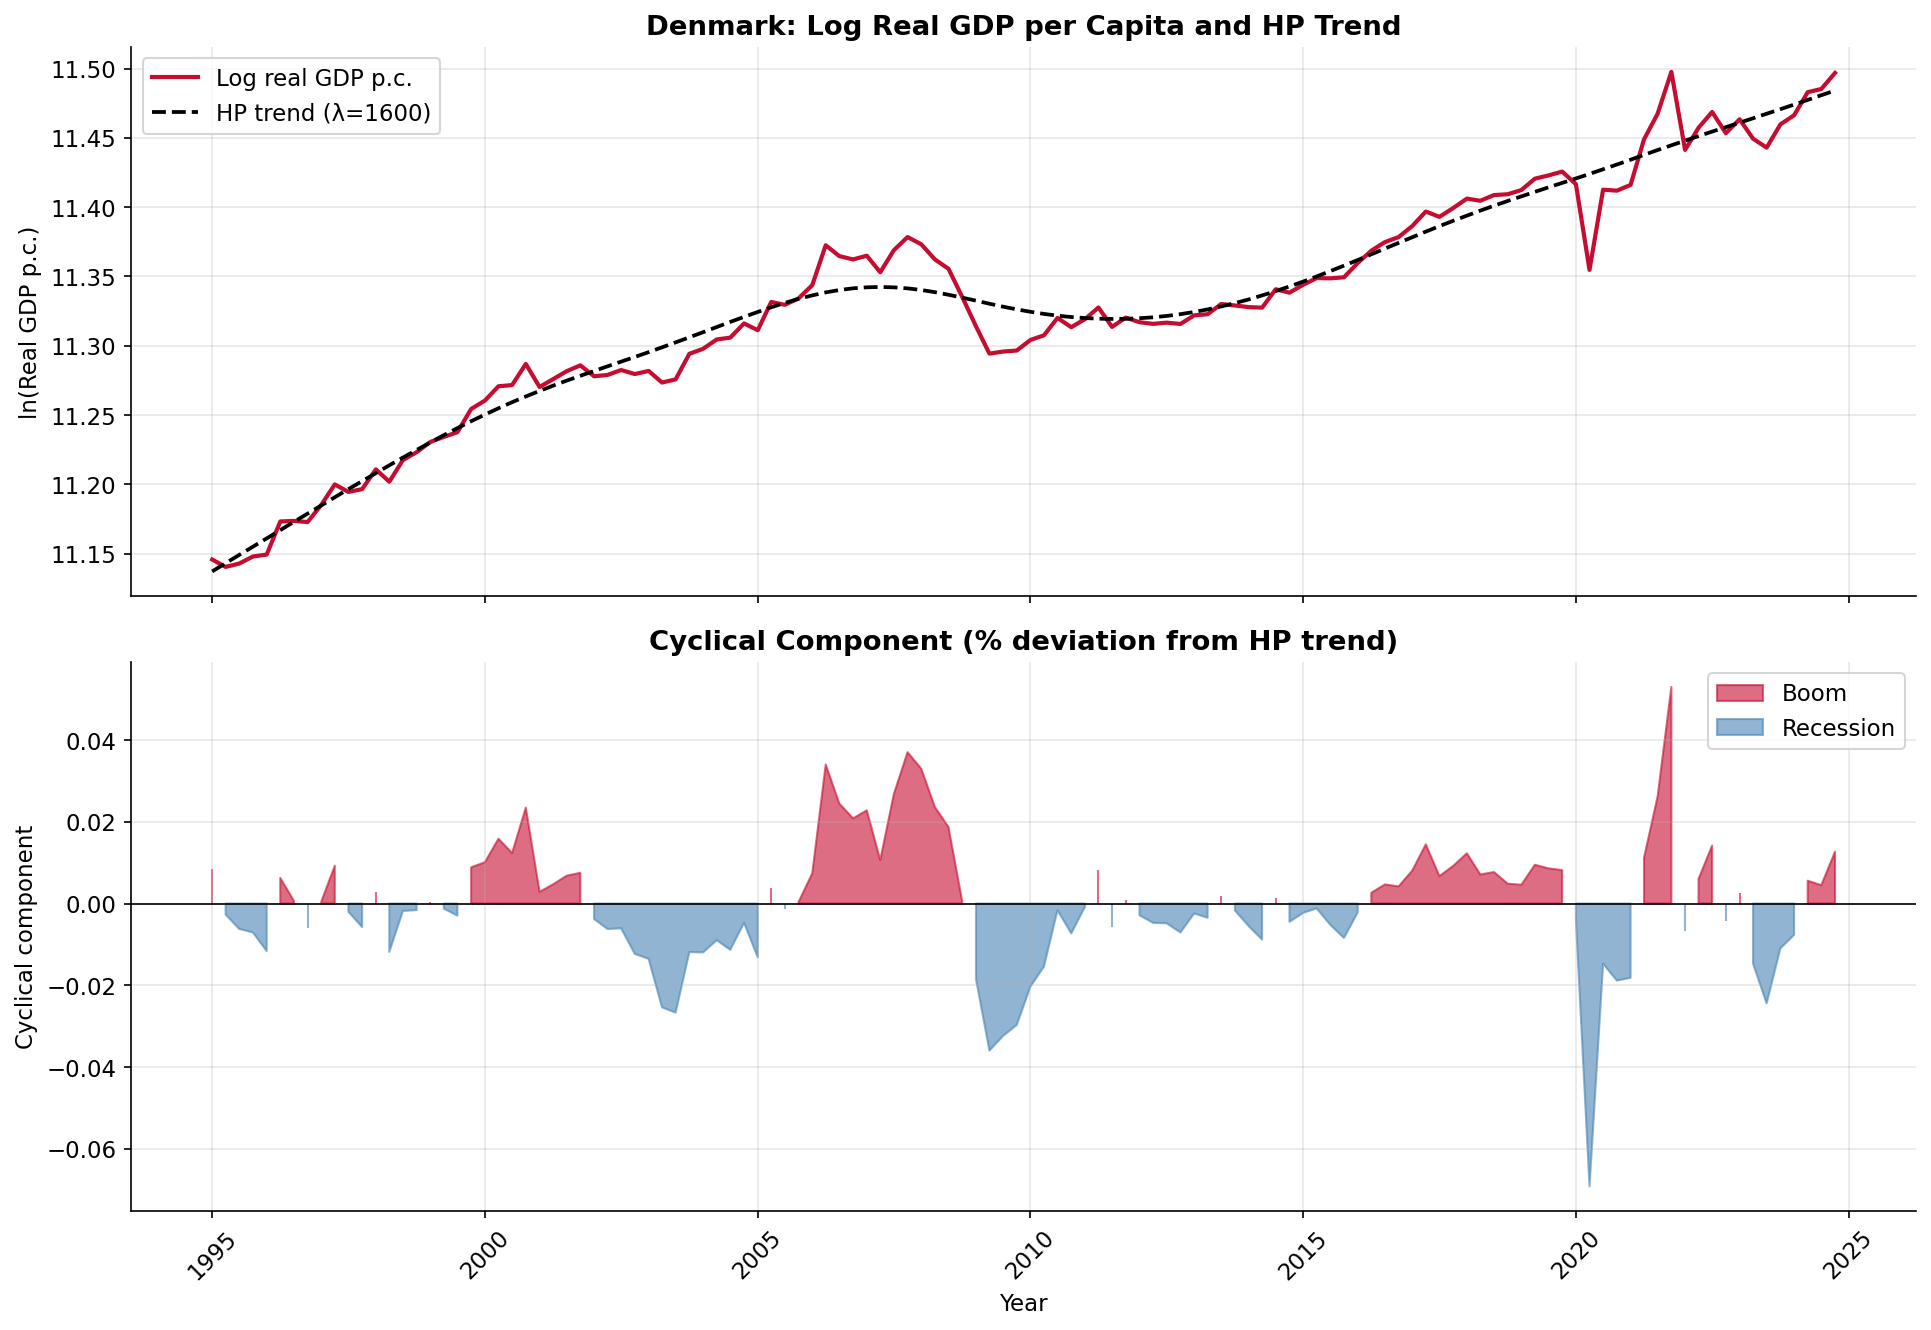
\includegraphics[width=\linewidth]{Denmark/denmark_hp_filter.png}
    \end{column}
    \begin{column}{0.48\textwidth}
      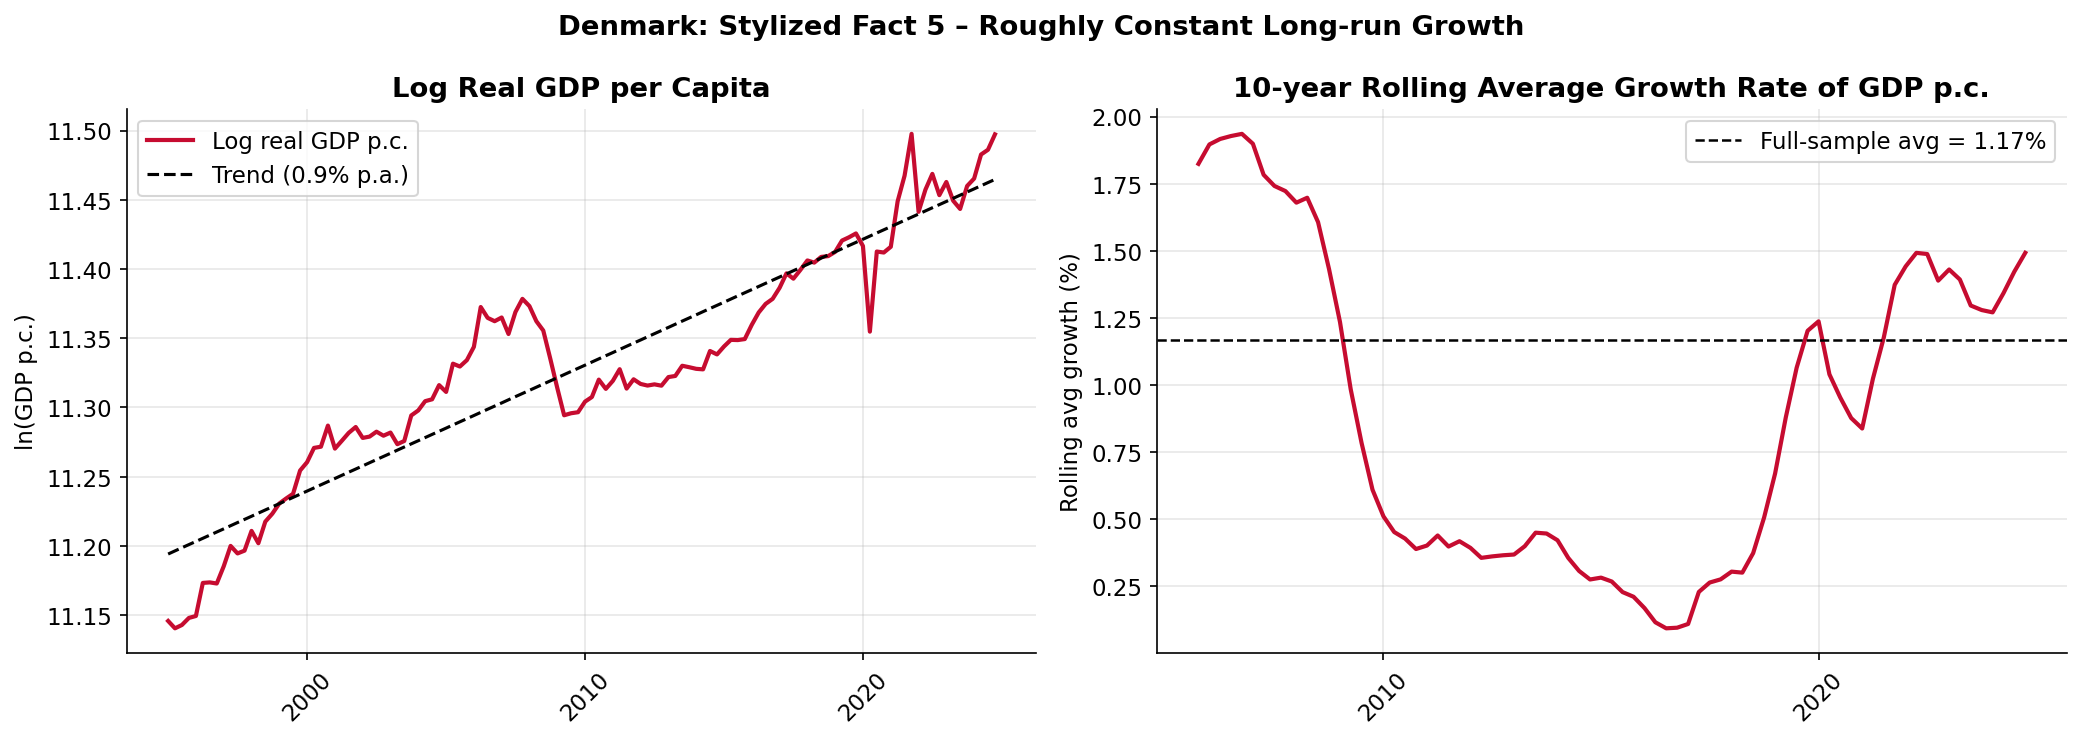
\includegraphics[width=\linewidth]{Denmark/denmark_stylized5.png}
    \end{column}
  \end{columns}
  \vspace{0.15cm}
  \small
  \begin{itemize}\setlength\itemsep{2pt}
    \item Output gap autocorrelation $\rho\approx0.84$ — persistent cycles
    \item Unemployment $\approx5\%$ average; CPI trend $\approx1.8\%$ since 2000
    \item Strong counter-cyclical unemployment; GFC spike to $\sim8\%$
  \end{itemize}
\end{frame}

% ── DK 3: Stylised Facts & Factor Shares ────────────────────
\begin{frame}{Denmark – Stylised Facts}
  \framesubtitle{SF1–SF7 from Kaldor; cross-country GDP comparison}
  \begin{columns}[T]
    \begin{column}{0.55\textwidth}
      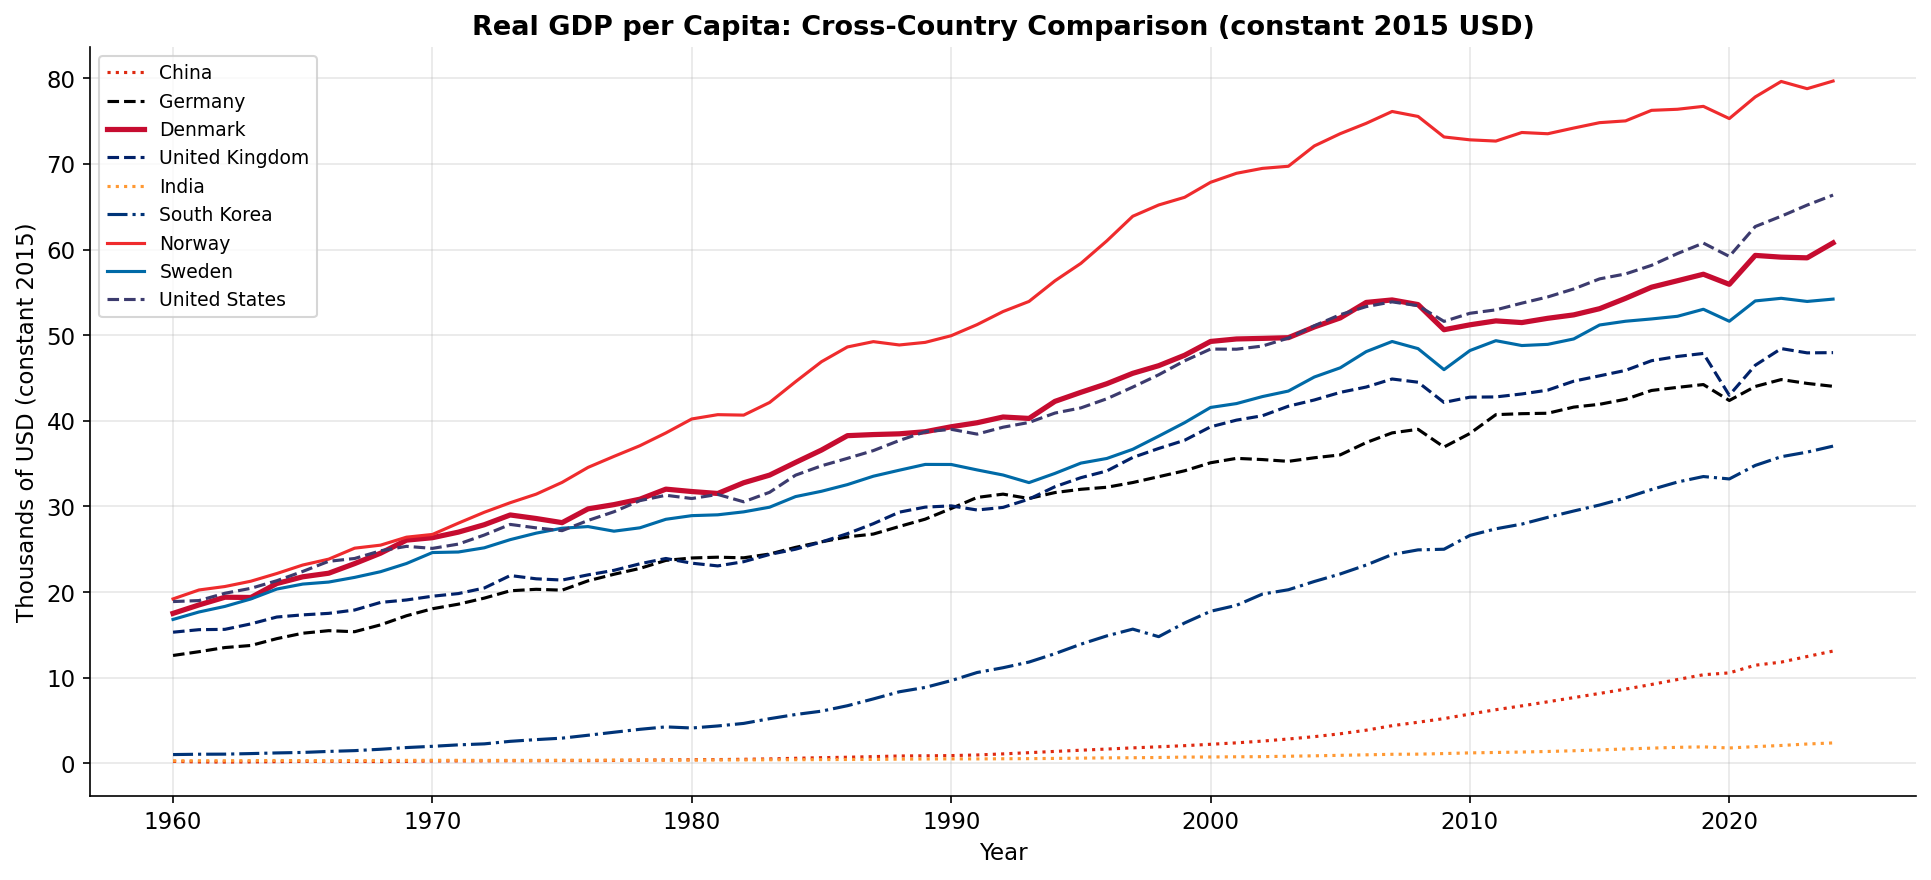
\includegraphics[width=\linewidth]{Denmark/denmark_cross_country_gdppc.png}
    \end{column}
    \begin{column}{0.42\textwidth}
      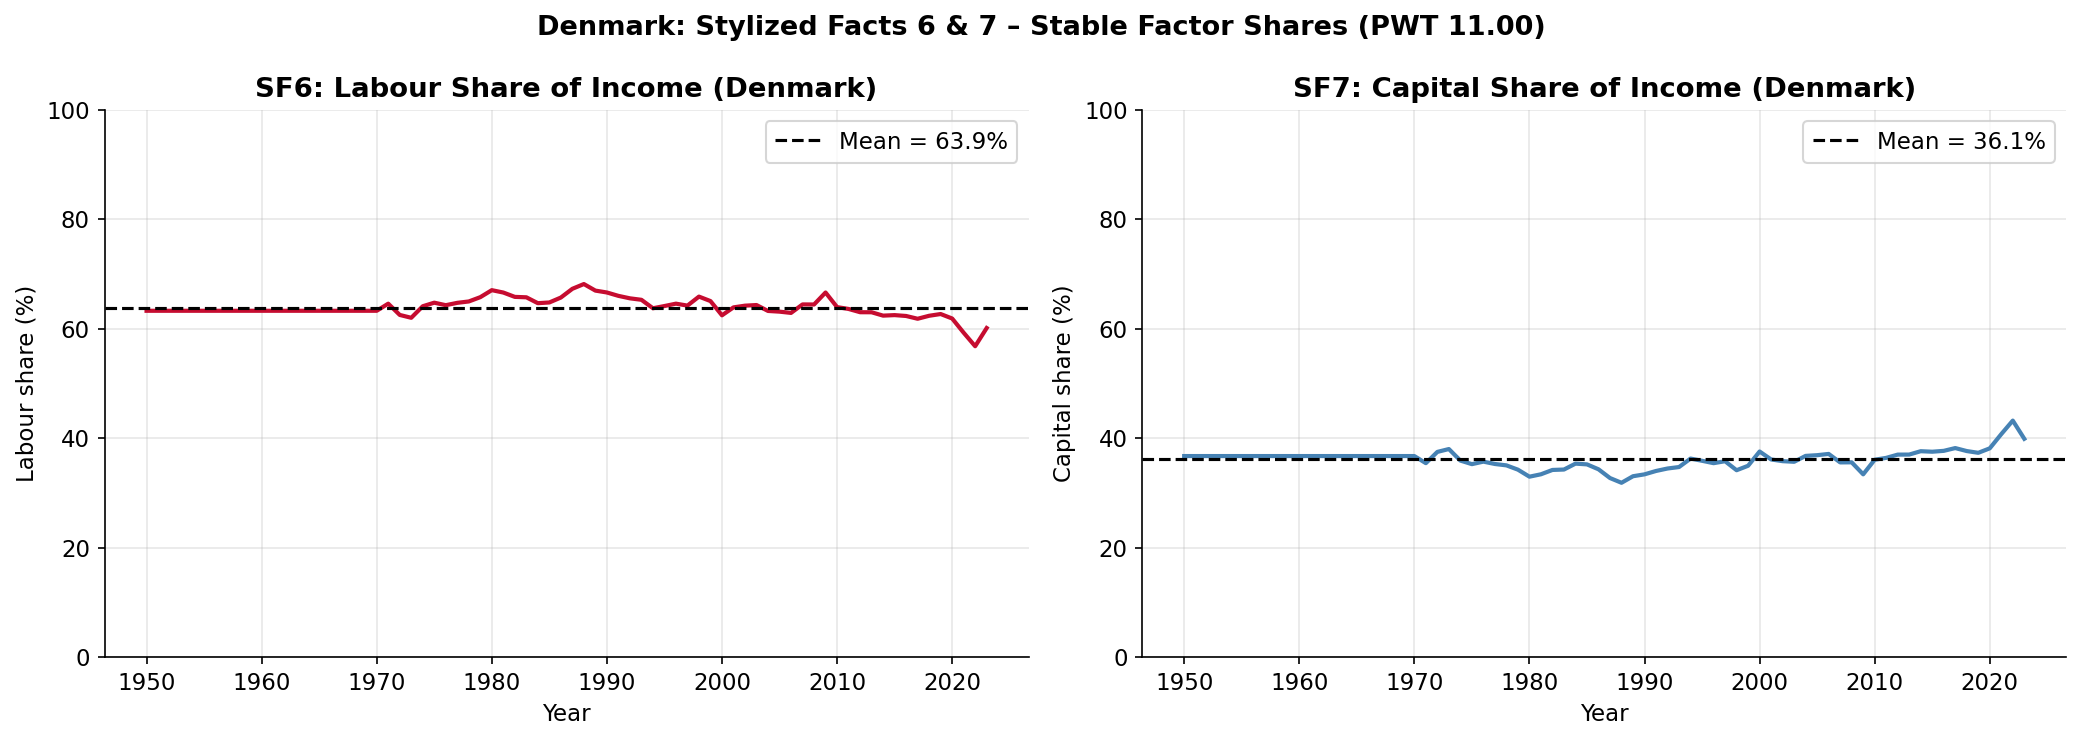
\includegraphics[width=\linewidth]{Denmark/denmark_factor_shares.png}
    \end{column}
  \end{columns}
  \vspace{0.1cm}
  \small
  \begin{itemize}\setlength\itemsep{2pt}
    \item Broadly confirms SF1–SF7: stable growth, balanced factor shares ($\alpha\approx0.37$)
    \item Labour share $\approx63\%$; capital share relatively stable — consistent with SF6/SF7
  \end{itemize}
\end{frame}

% ── DK 4: Solow Model ───────────────────────────────────────
\begin{frame}{Denmark – Solow Model}
  \framesubtitle{PWT calibration 2000–2019; savings shock $s\uparrow$}
  \begin{columns}[T]
    \begin{column}{0.58\textwidth}
      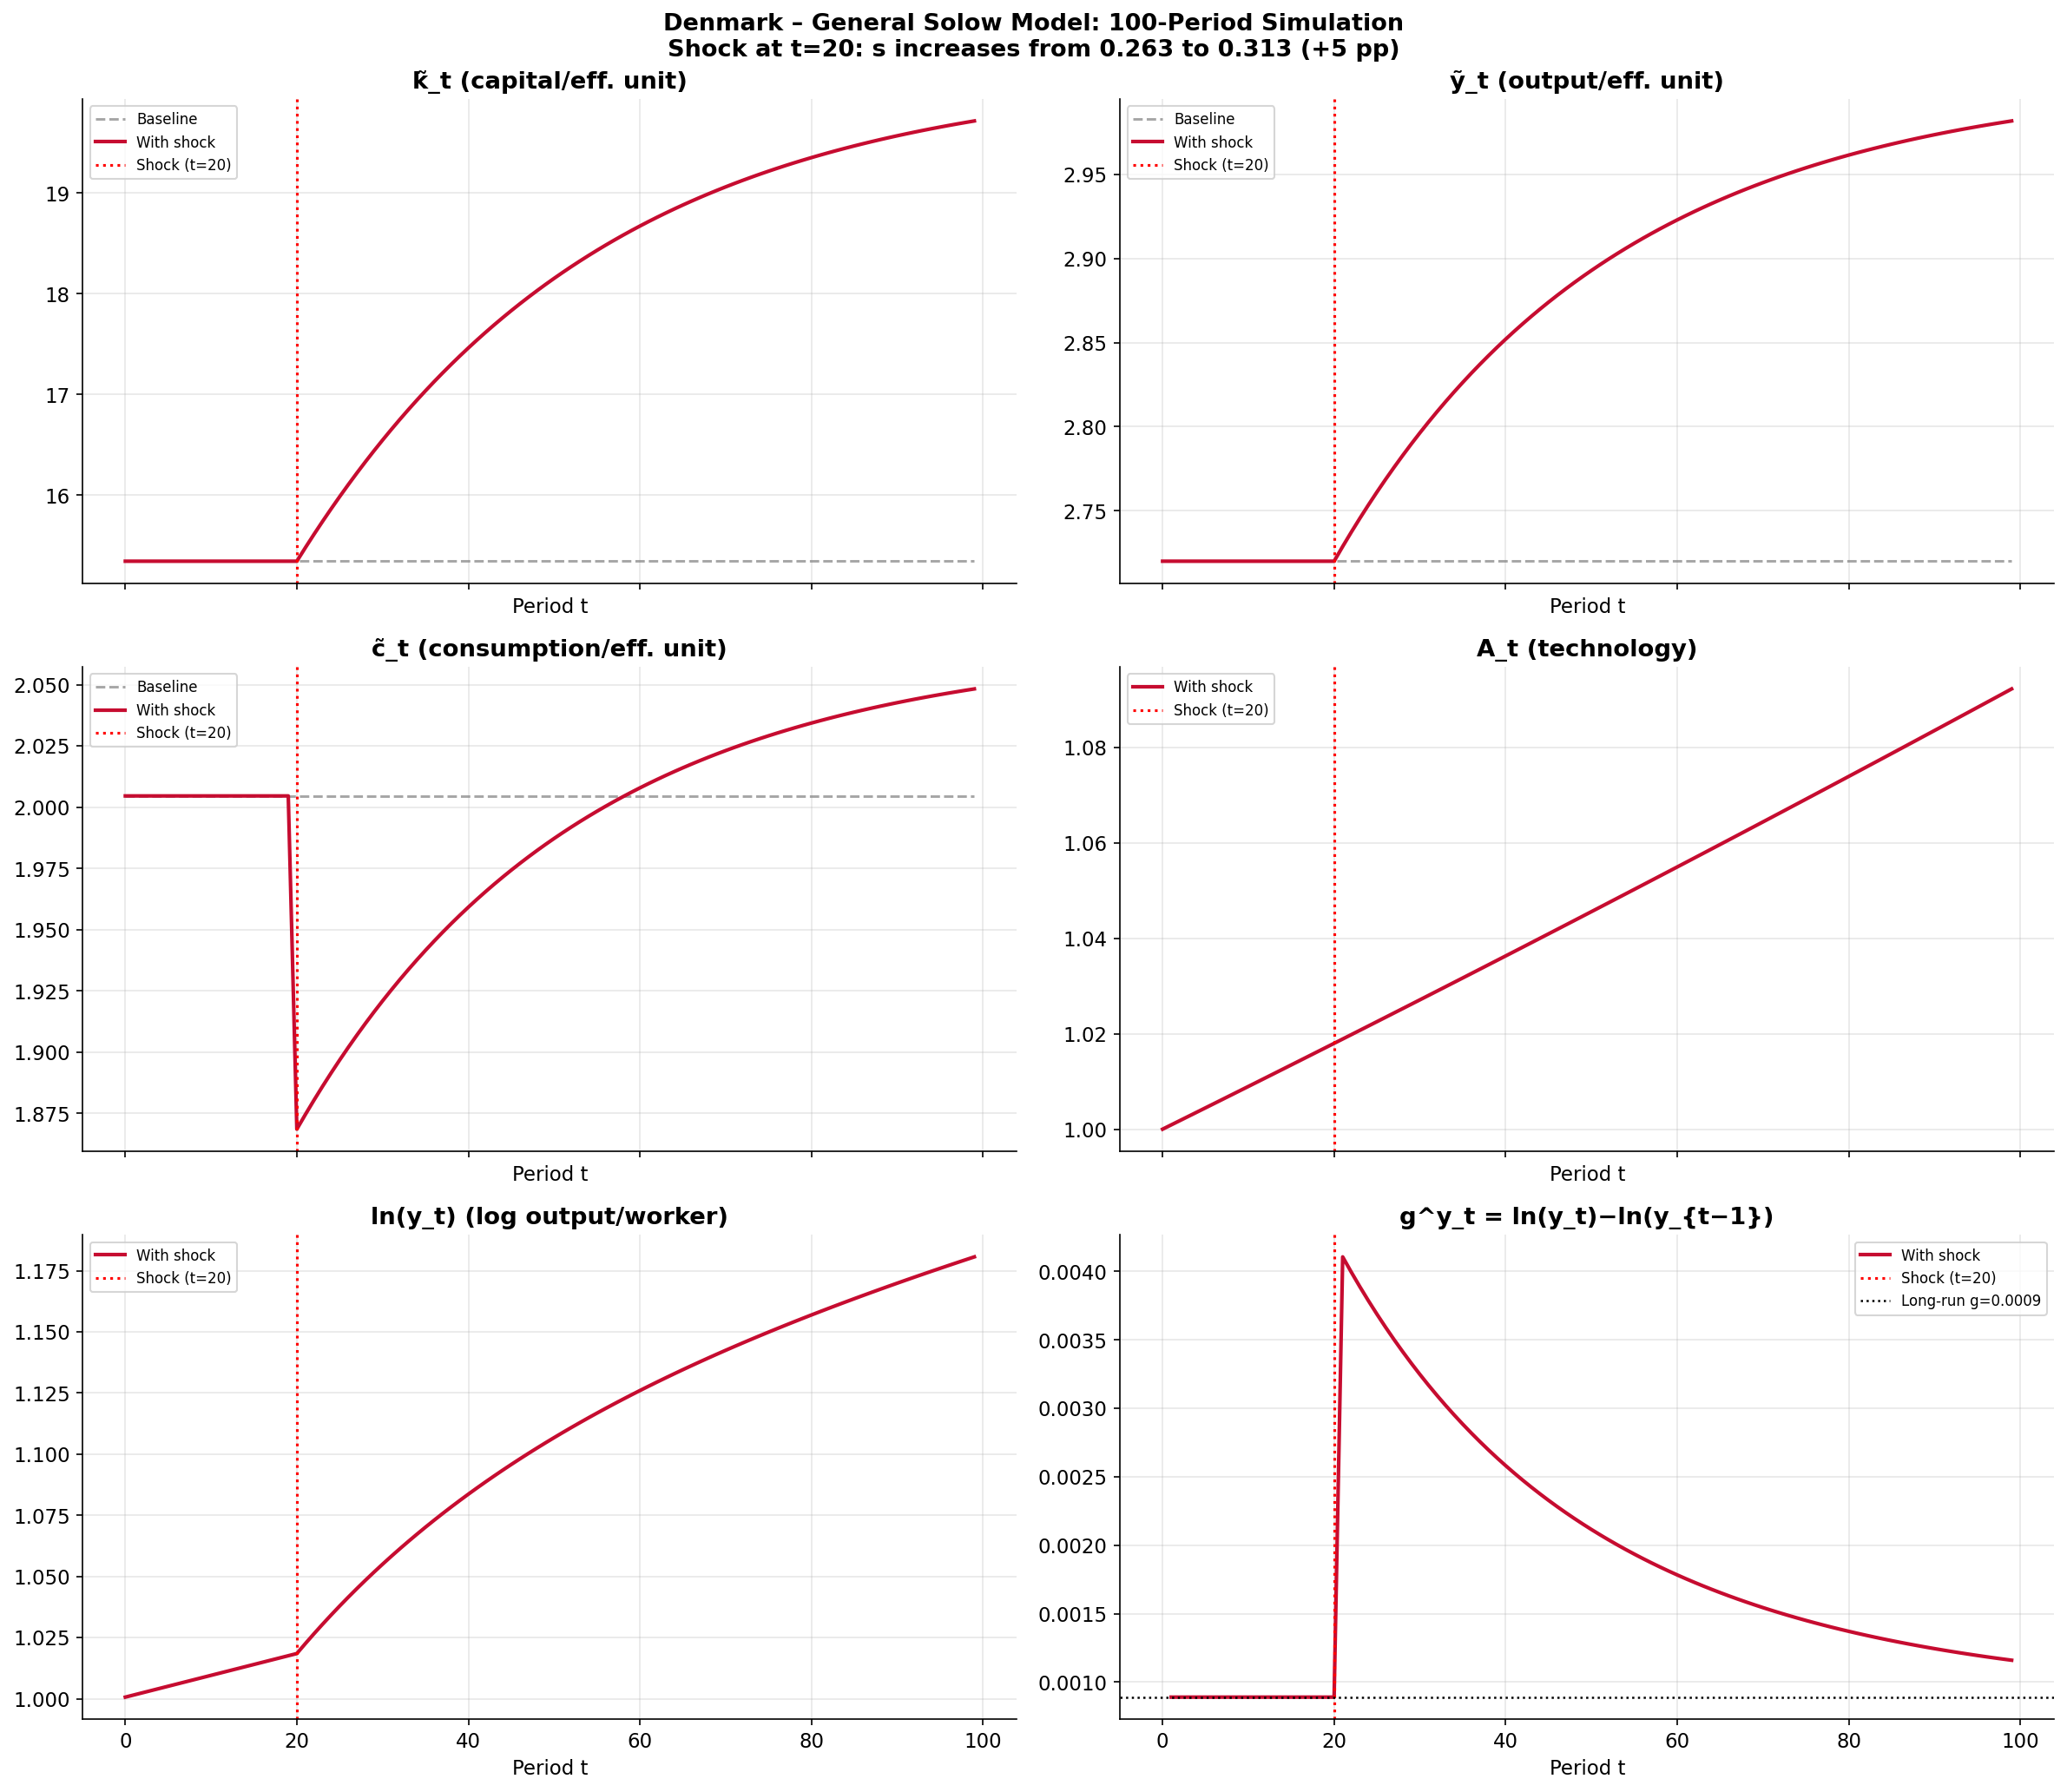
\includegraphics[width=\linewidth]{Denmark/denmark_solow_overview.png}
    \end{column}
    \begin{column}{0.39\textwidth}
      \vspace{0.3cm}
      \small
      \begin{tabular}{@{}Lr@{}}
        \toprule
        \textbf{Parameter} & \textbf{Value} \\
        \midrule
        $\alpha$ & 0.366 \\
        $s$      & 0.263 \\
        $\delta$ & 0.041 \\
        $n$      & 0.005 \\
        $g$      & 0.001 \\
        \midrule
        $\tilde{k}^*$ & 15.35 \\
        $\tilde{y}^*$ & 2.72 \\
        \bottomrule
      \end{tabular}
      \vspace{0.4cm}
      \begin{itemize}\setlength\itemsep{3pt}
        \item $s<\alpha$: below Golden Rule
        \item Savings $\uparrow\Rightarrow\tilde{c}^*\uparrow$ (welfare gain)
        \item Smooth transition to new SS
      \end{itemize}
    \end{column}
  \end{columns}
\end{frame}

% ============================================================
%  PART 2 – NORWAY
% ============================================================
\sectionslide{norred}{Norway}{\textcolor{white!70!norred}{Oil Economy \& Solow Anomalies}}

% ── NO 1: GDP per capita ────────────────────────────────────
\begin{frame}{Norway – GDP per Capita}
  \framesubtitle{Trend growth $\approx1.0\%$ p.a. since 2000 (1978 Q1 – 2024 Q4)}
  \begin{columns}[T]
    \begin{column}{0.62\textwidth}
      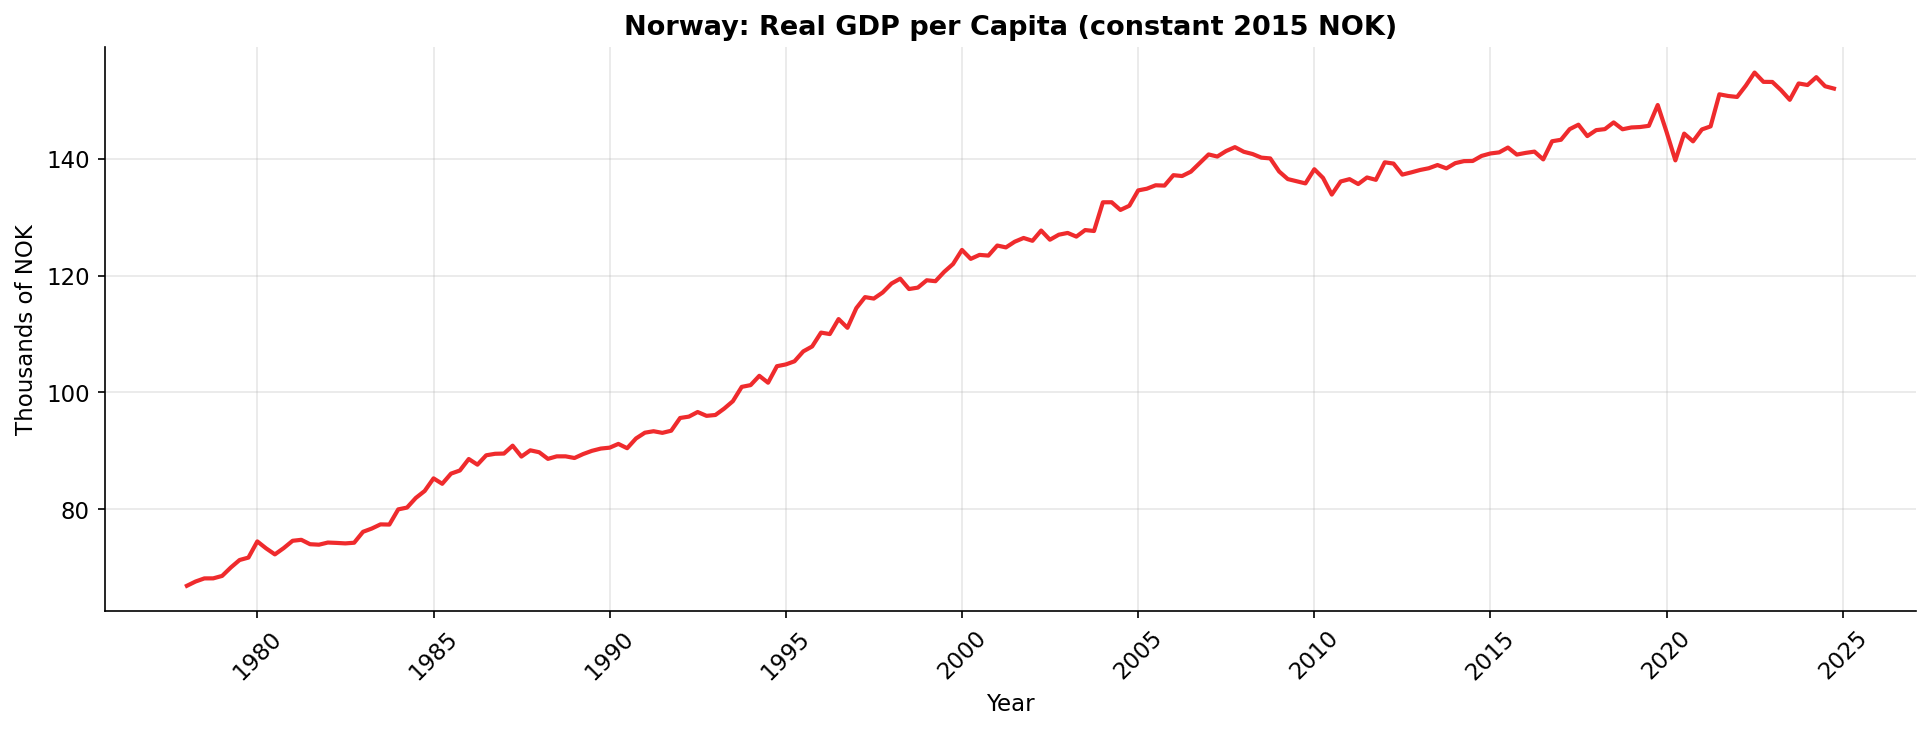
\includegraphics[width=\linewidth]{Norway/norway_gdp_pc_level.png}
    \end{column}
    \begin{column}{0.35\textwidth}
      \vspace{0.3cm}
      \small
      \begin{tabular}{@{}Lr@{}}
        \toprule
        \textbf{Indicator} & \textbf{Value} \\
        \midrule
        Sample & 1978–2024 \\
        Trend growth & $\approx1.0\%$ p.a. \\
        Oil shock 2015–16 & mild dip \\
        COVID drop & $\approx-3\%$ \\
        \bottomrule
      \end{tabular}
      \vspace{0.5cm}
      \begin{itemize}\setlength\itemsep{3pt}
        \item Highest GDP/capita of three countries
        \item 1987–89 banking crisis trough
        \item Oil wealth buffers recessions
      \end{itemize}
    \end{column}
  \end{columns}
\end{frame}

% ── NO 2: Business Cycles ───────────────────────────────────
\begin{frame}{Norway – Business Cycles}
  \framesubtitle{HP-filtered output gap · lowest output volatility ($\sigma=0.013$)}
  \begin{columns}[T]
    \begin{column}{0.48\textwidth}
      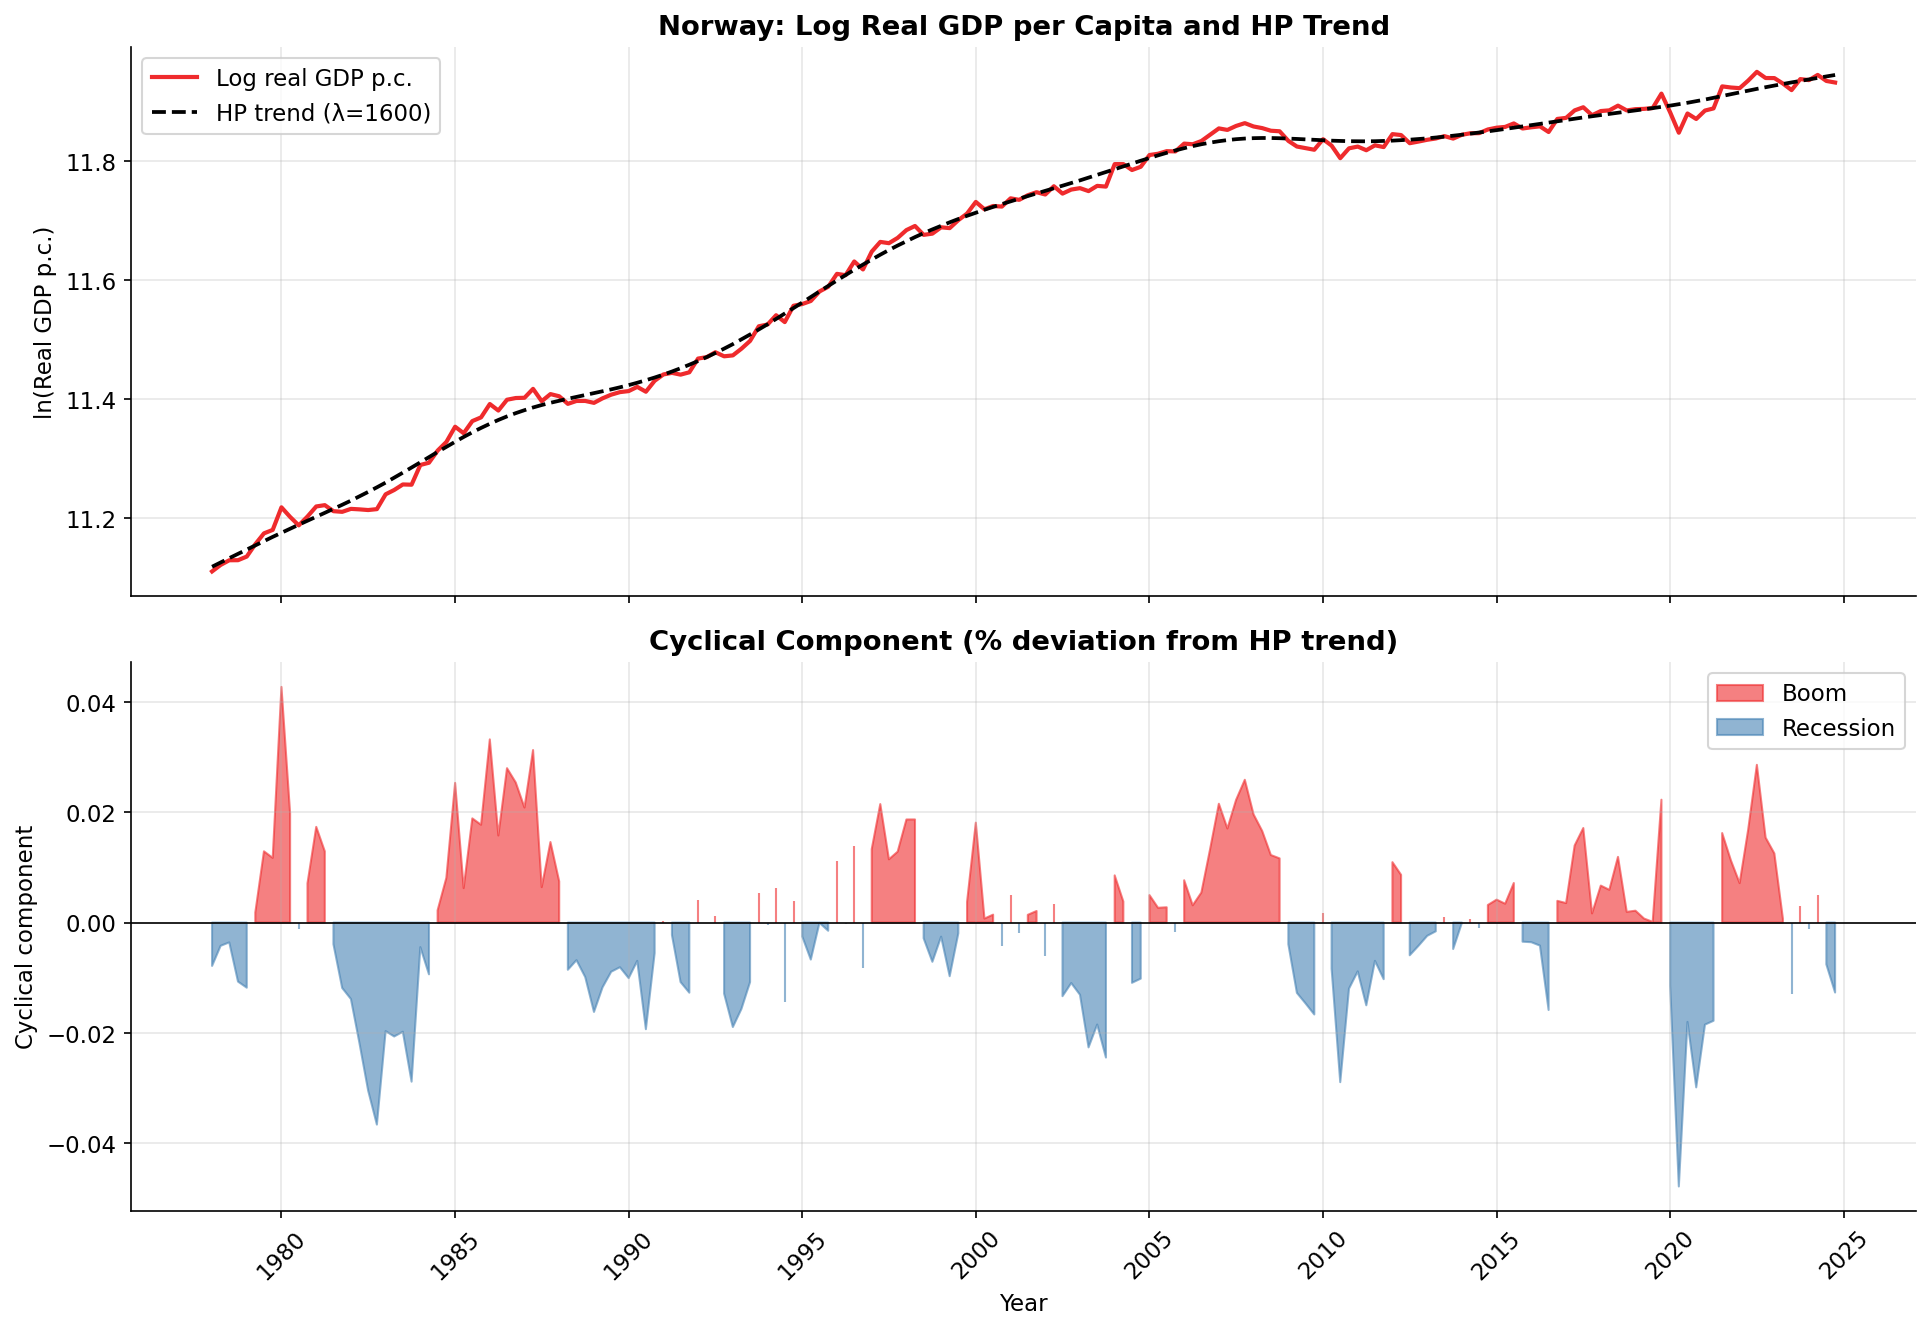
\includegraphics[width=\linewidth]{Norway/norway_hp_filter.png}
    \end{column}
    \begin{column}{0.48\textwidth}
      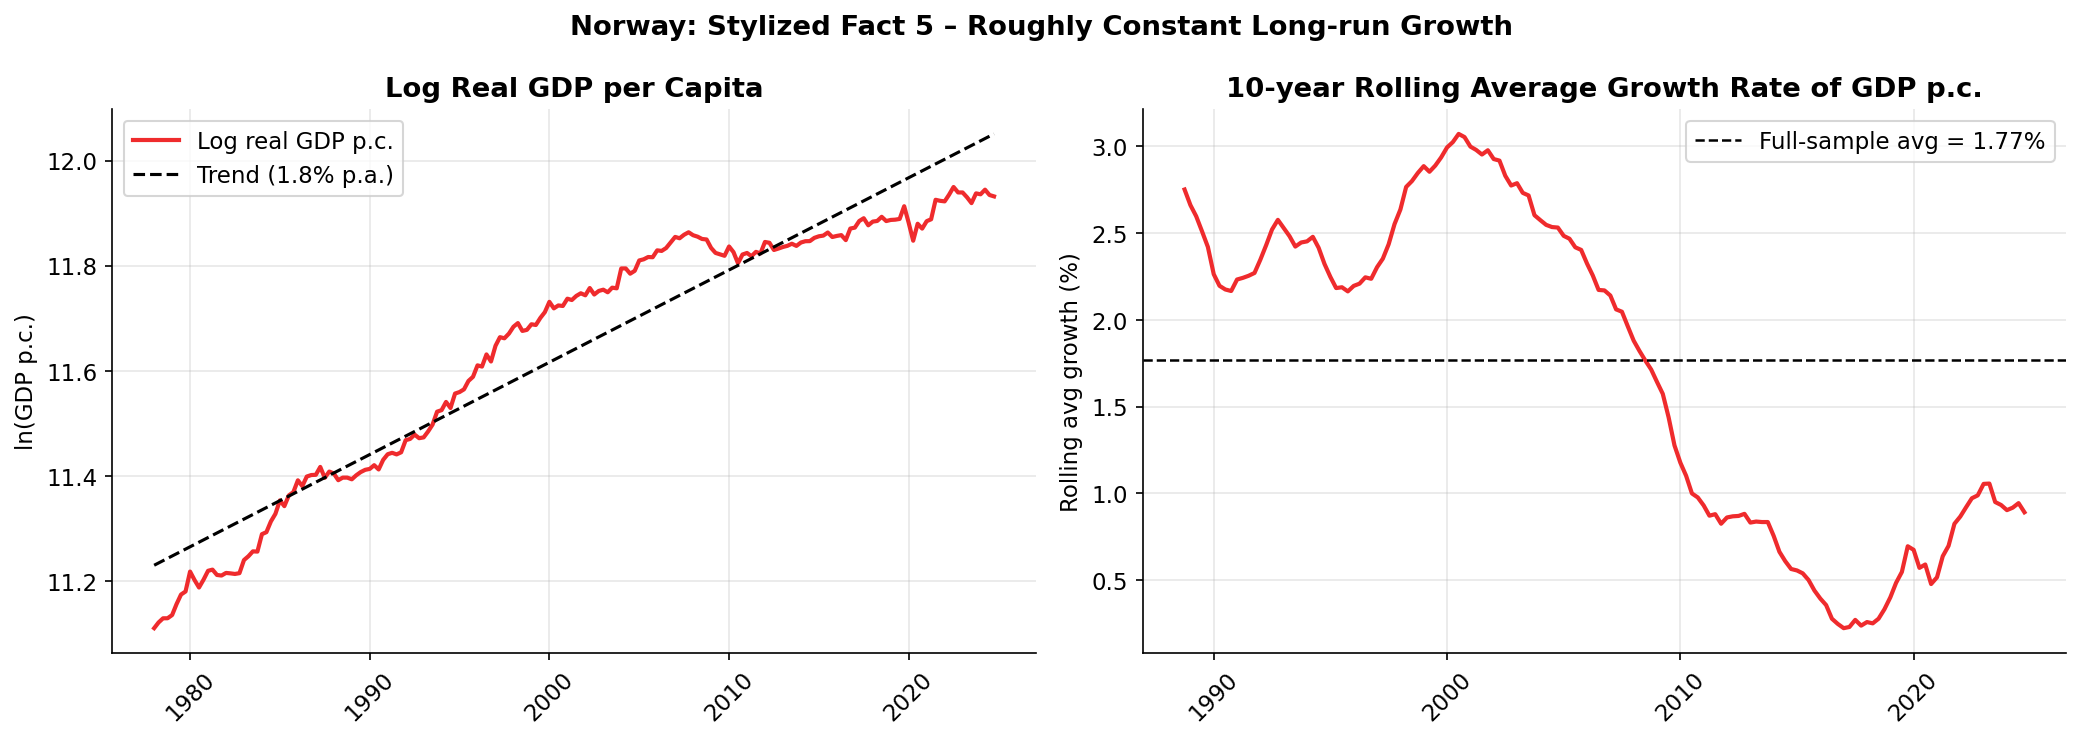
\includegraphics[width=\linewidth]{Norway/norway_stylized5.png}
    \end{column}
  \end{columns}
  \vspace{0.15cm}
  \small
  \begin{itemize}\setlength\itemsep{2pt}
    \item Output autocorrelation $\rho\approx0.60$ — moderate persistence
    \item Unemployment $\approx3.7\%$ avg since 2000 — lowest of three countries
    \item CPI $\approx2.5\%$ since 2000; oil fund stabilises fiscal cycle
  \end{itemize}
\end{frame}

% ── NO 3: Oil Anomalies & Factor Shares ─────────────────────
\begin{frame}{Norway – Oil Anomalies}
  \framesubtitle{Factor shares violate SF6/SF7; $\alpha=0.505$ driven by oil rents}
  \begin{columns}[T]
    \begin{column}{0.55\textwidth}
      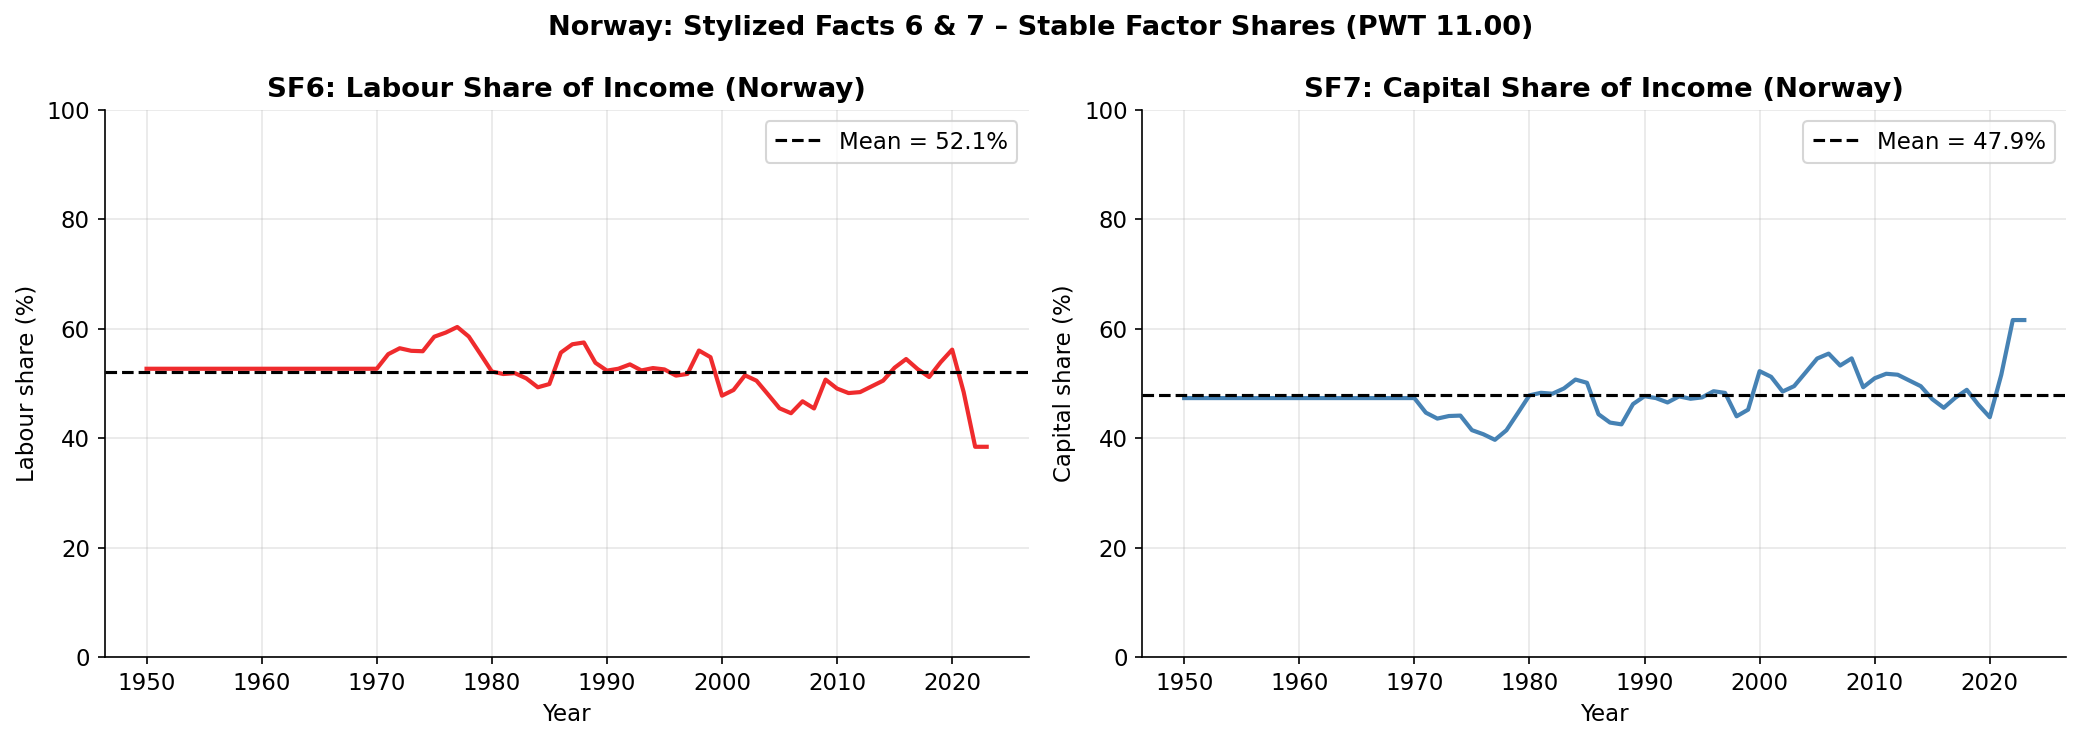
\includegraphics[width=\linewidth]{Norway/norway_factor_shares.png}
    \end{column}
    \begin{column}{0.42\textwidth}
      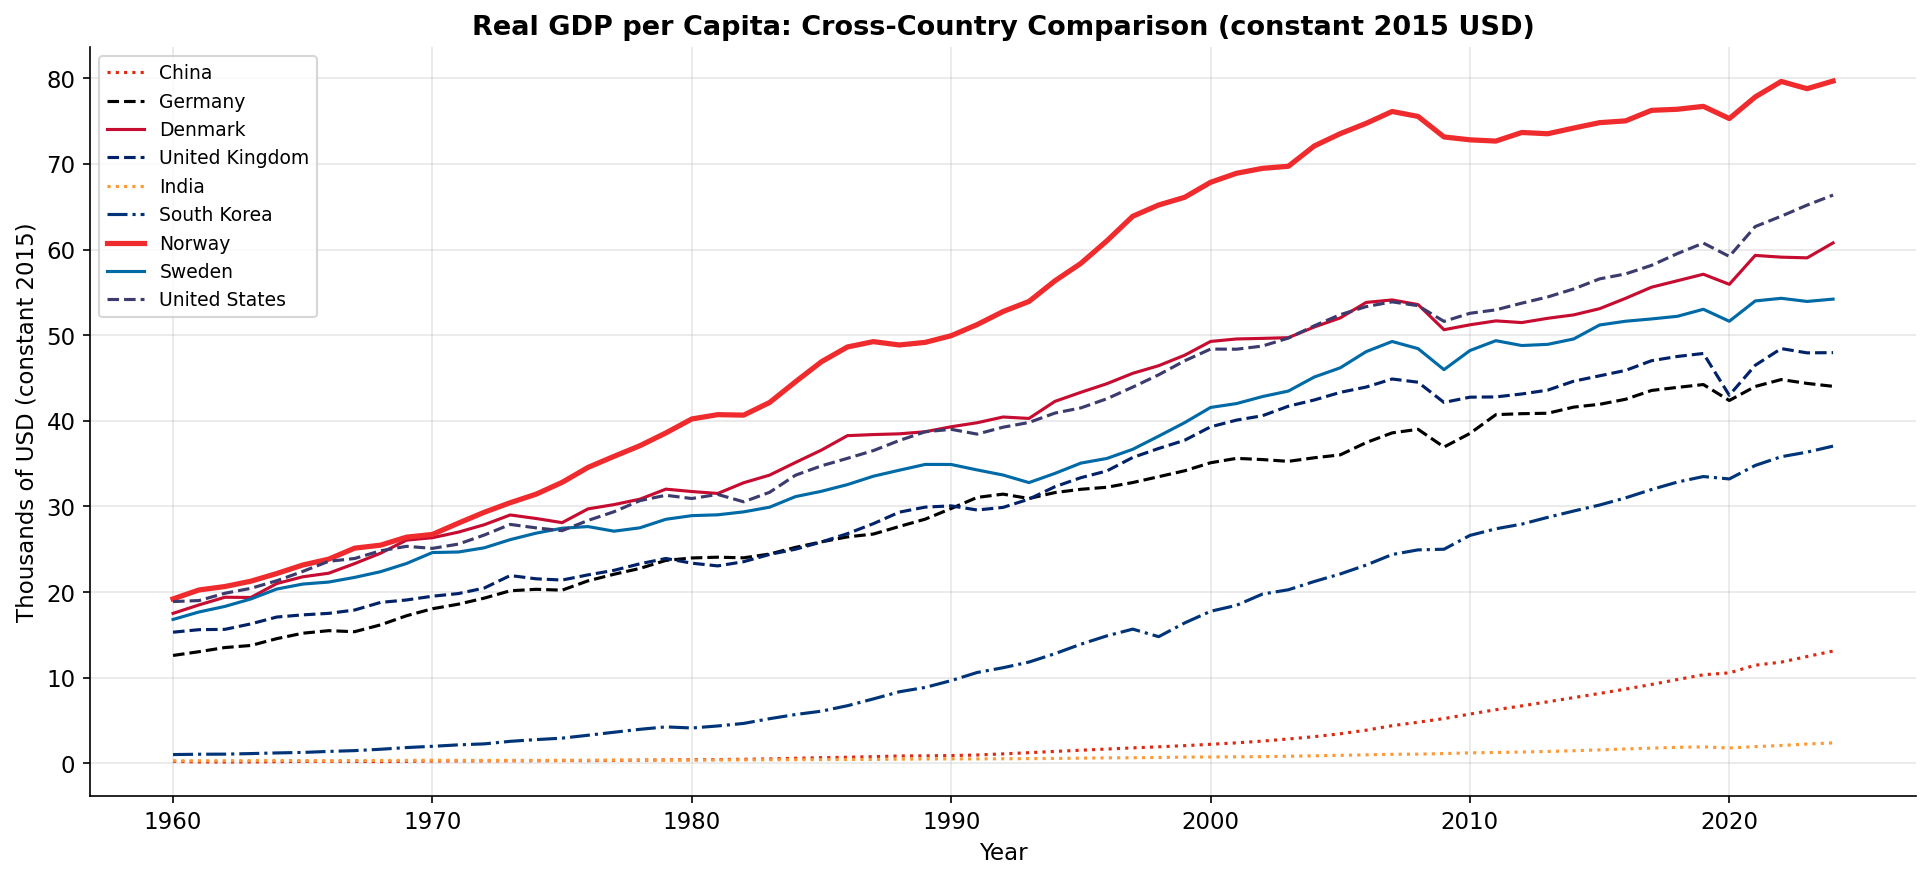
\includegraphics[width=\linewidth]{Norway/norway_cross_country_gdppc.png}
    \end{column}
  \end{columns}
  \vspace{0.1cm}
  \small
  \begin{itemize}\setlength\itemsep{2pt}
    \item Labour share swings \textbf{38\%–65\%} with oil price cycle — violates SF6/SF7
    \item Norway well above peer-group trajectory: oil-wealth premium
  \end{itemize}
\end{frame}

% ── NO 4: Solow Model ───────────────────────────────────────
\begin{frame}{Norway – Solow Model}
  \framesubtitle{PWT calibration 2000–2019; Oil Fund fiscal rule shock}
  \begin{columns}[T]
    \begin{column}{0.58\textwidth}
      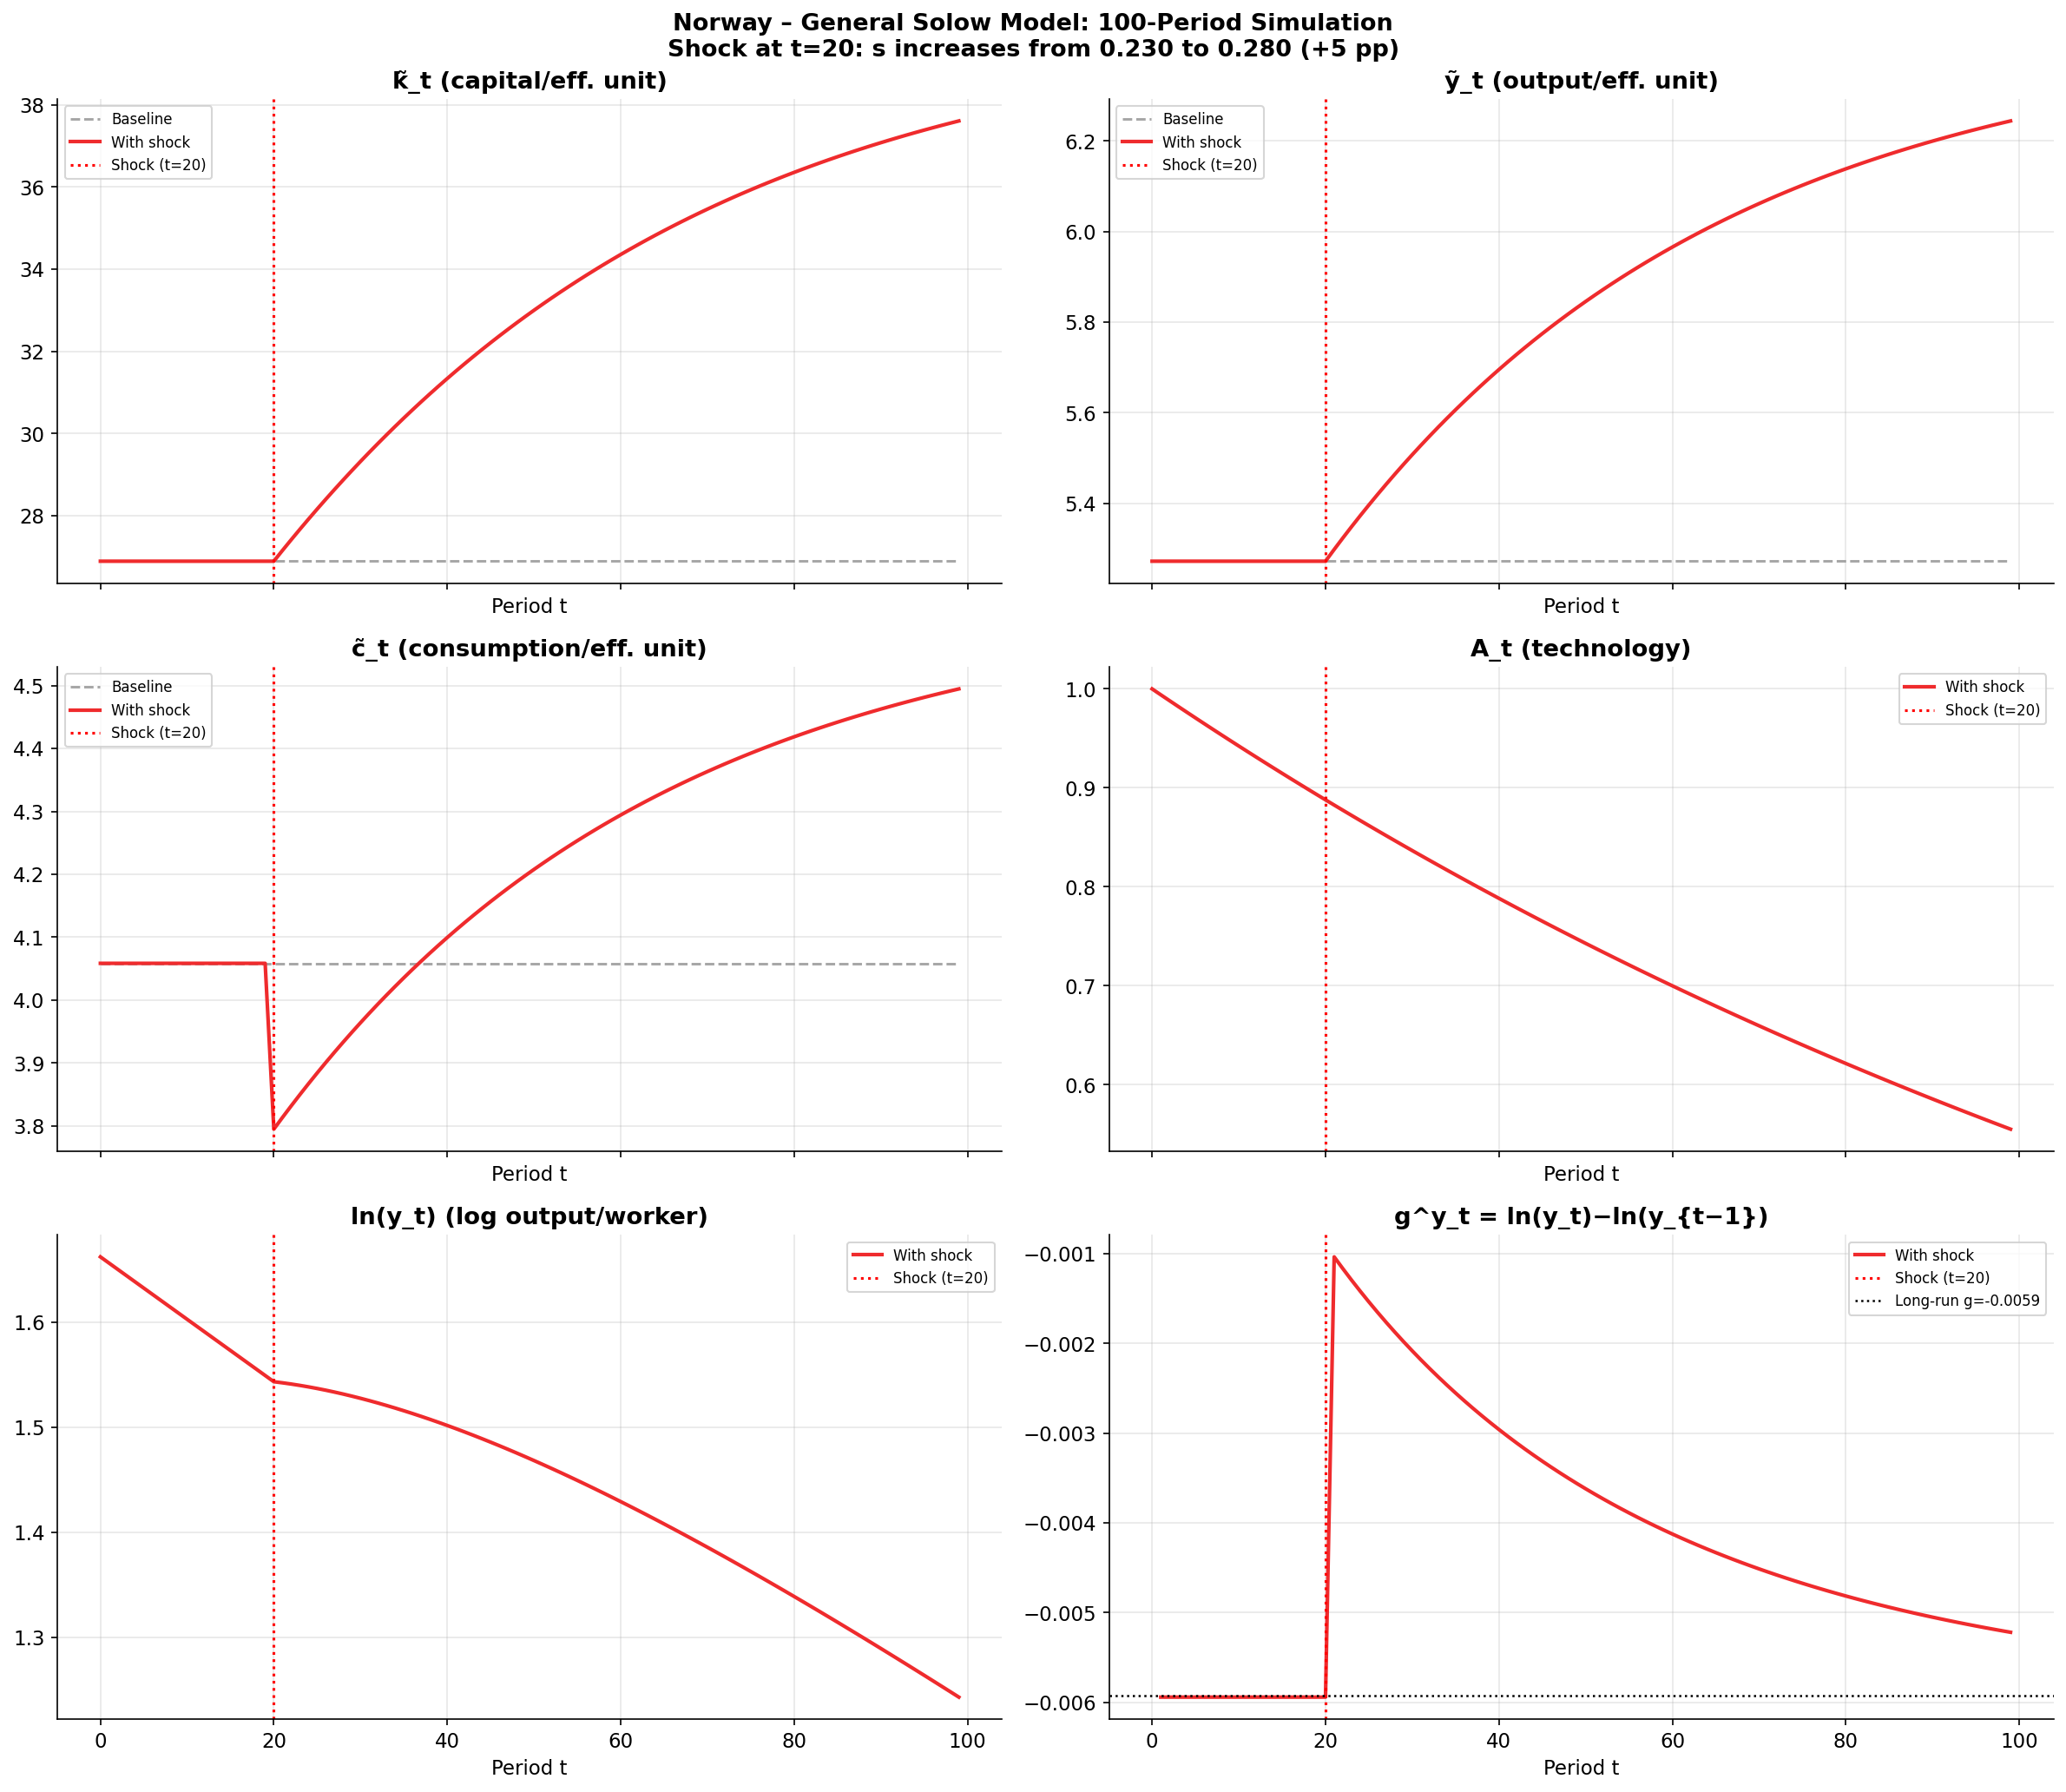
\includegraphics[width=\linewidth]{Norway/norway_solow_overview.png}
    \end{column}
    \begin{column}{0.39\textwidth}
      \vspace{0.3cm}
      \small
      \begin{tabular}{@{}Lr@{}}
        \toprule
        \textbf{Parameter} & \textbf{Value} \\
        \midrule
        $\alpha$ & 0.505 \\
        $s$      & 0.230 \\
        $\delta$ & 0.042 \\
        $n$      & 0.009 \\
        $g$      & $-0.006$ \\
        \midrule
        $\tilde{k}^*$ & 26.90 \\
        $\tilde{y}^*$ & 5.27 \\
        \bottomrule
      \end{tabular}
      \vspace{0.4cm}
      \begin{itemize}\setlength\itemsep{3pt}
        \item $g<0$: maturing oil fields
        \item $\alpha>0.5$: oil-inflated capital share
        \item Shock: reinvest more via GPFG ($s\uparrow$)
      \end{itemize}
    \end{column}
  \end{columns}
\end{frame}

% ============================================================
%  PART 3 – SWEDEN
% ============================================================
\sectionslide{sweblue}{Sweden}{\textcolor{white!70!sweblue}{ERM Crisis Legacy \& High Volatility}}

% ── SE 1: GDP per capita ────────────────────────────────────
\begin{frame}{Sweden – GDP per Capita}
  \framesubtitle{Trend growth $\approx1.25\%$ p.a. since 2000 (1993 Q1 – 2024 Q4)}
  \begin{columns}[T]
    \begin{column}{0.62\textwidth}
      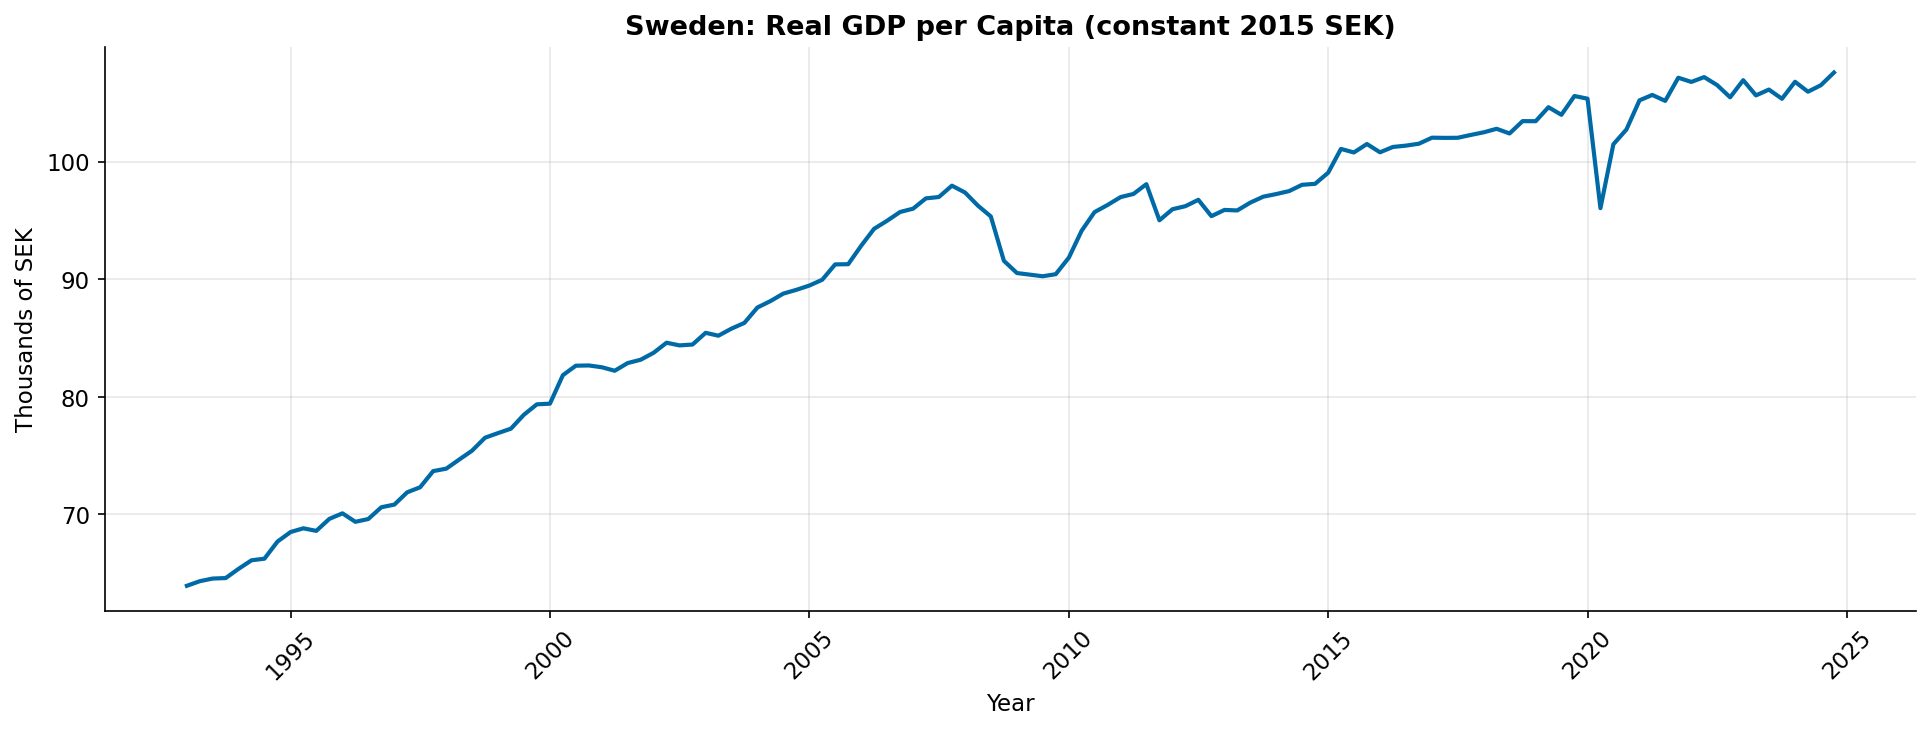
\includegraphics[width=\linewidth]{Sweden/sweden_gdp_pc_level.png}
    \end{column}
    \begin{column}{0.35\textwidth}
      \vspace{0.3cm}
      \small
      \begin{tabular}{@{}Lr@{}}
        \toprule
        \textbf{Indicator} & \textbf{Value} \\
        \midrule
        Sample & 1993–2024 \\
        Trend growth & $\approx1.25\%$ p.a. \\
        GFC drop & $\approx-7\%$ \\
        COVID drop & $\approx-8\%$ \\
        \bottomrule
      \end{tabular}
      \vspace{0.5cm}
      \begin{itemize}\setlength\itemsep{3pt}
        \item Fastest-growing of the three countries
        \item Deepest COVID contraction in sample
        \item Strong post-GFC V-shaped recovery
      \end{itemize}
    \end{column}
  \end{columns}
\end{frame}

% ── SE 2: Business Cycles ───────────────────────────────────
\begin{frame}{Sweden – Business Cycles}
  \framesubtitle{Highest output volatility ($\sigma=0.018$) · Unemployment \& Inflation}
  \begin{columns}[T]
    \begin{column}{0.48\textwidth}
      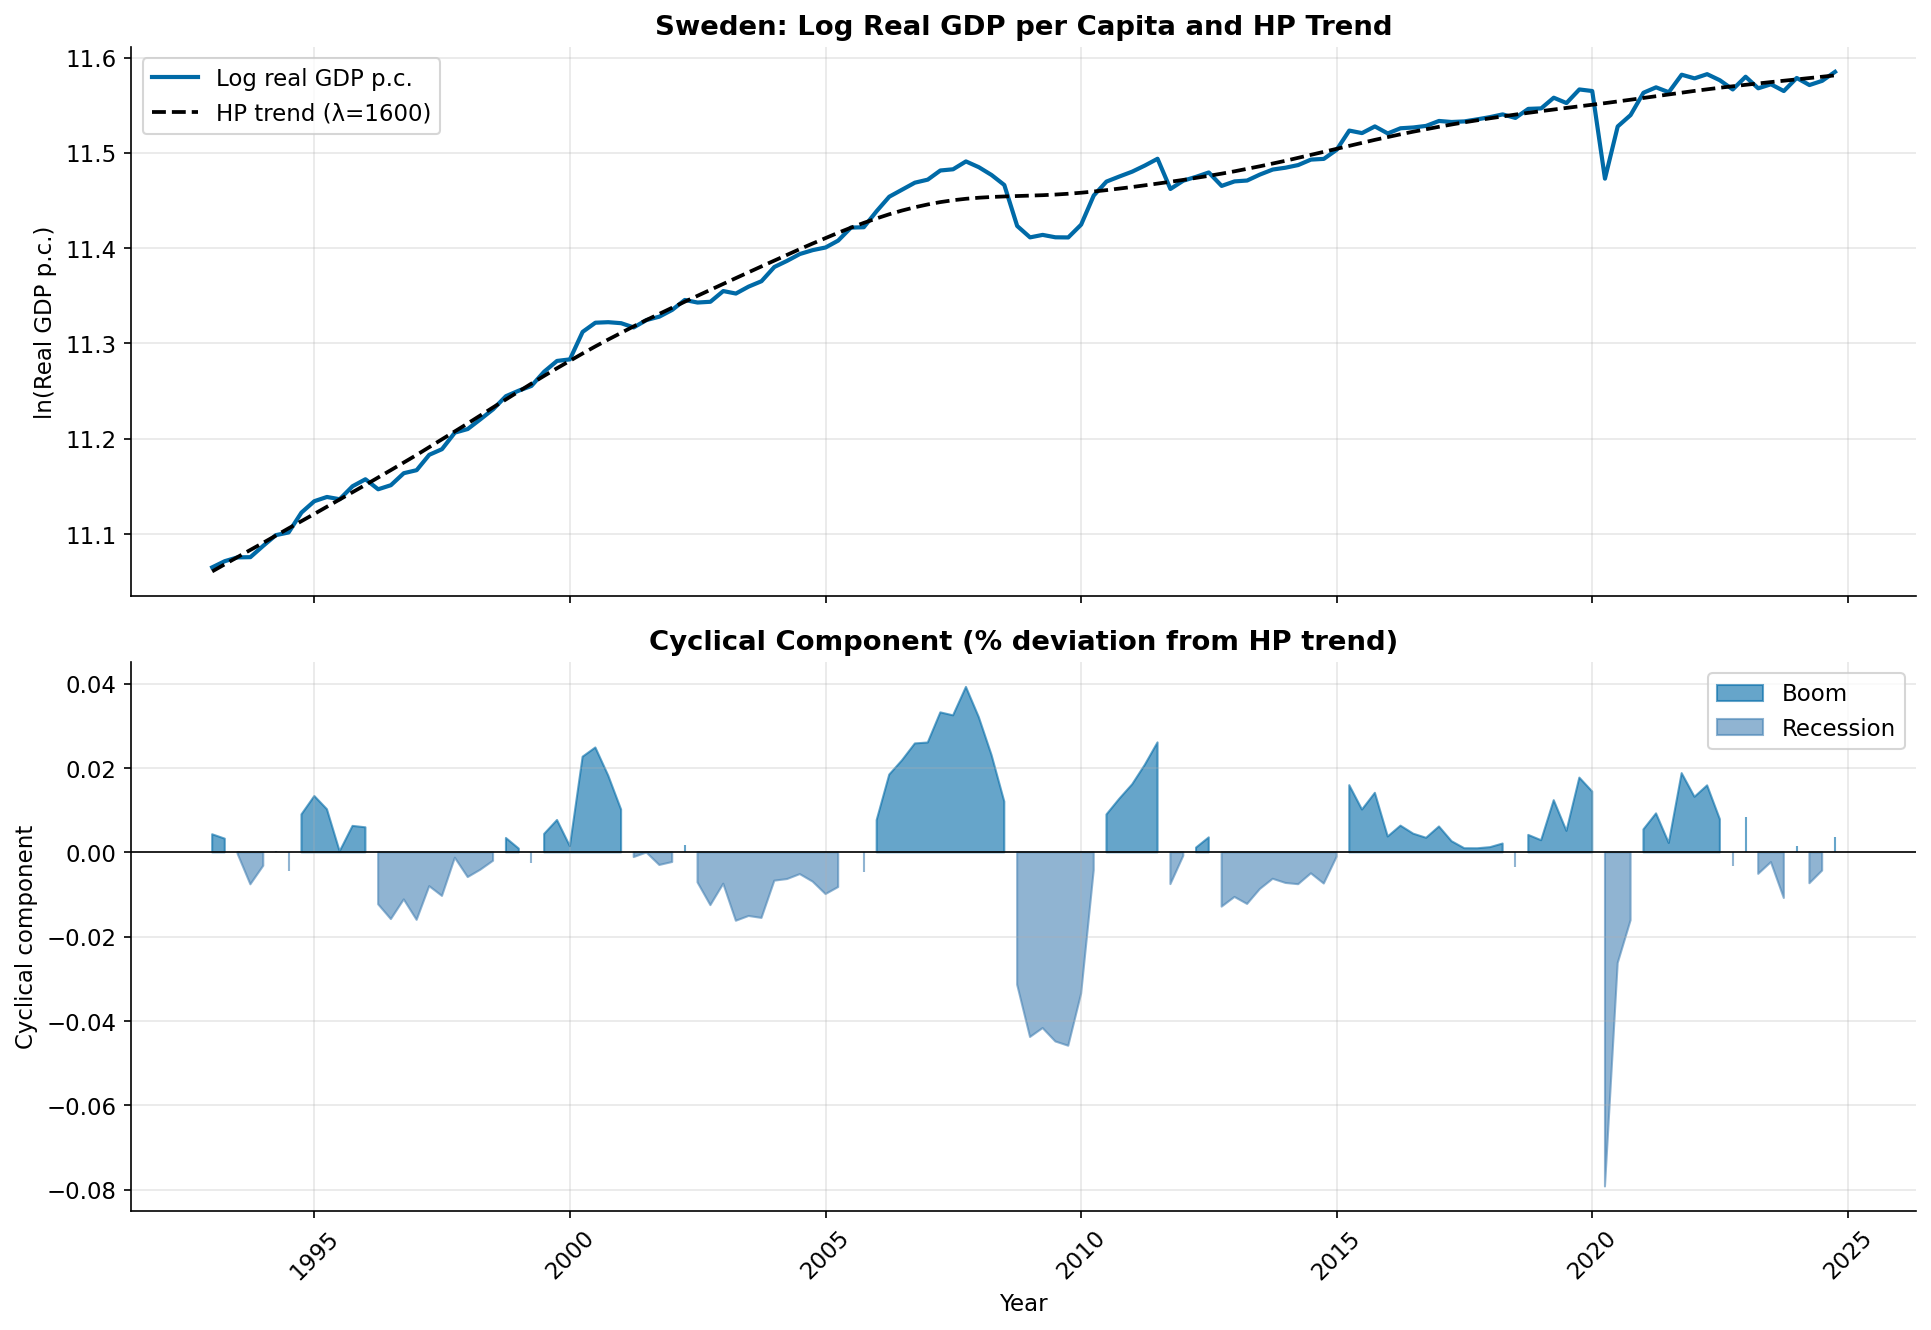
\includegraphics[width=\linewidth]{Sweden/sweden_hp_filter.png}
    \end{column}
    \begin{column}{0.48\textwidth}
      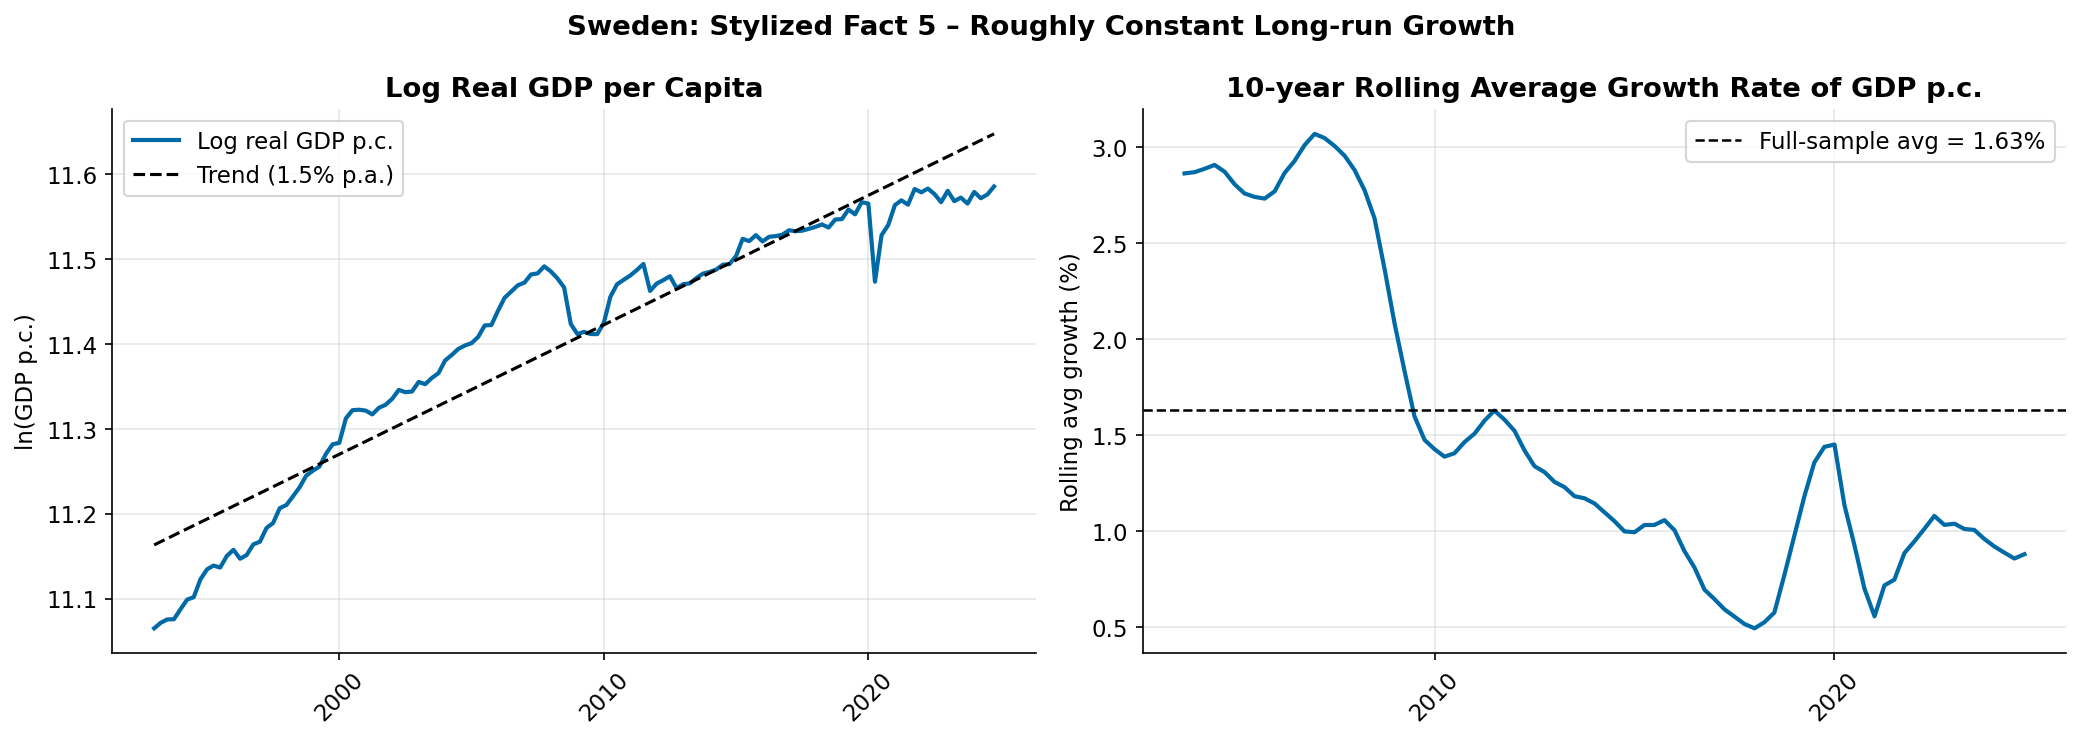
\includegraphics[width=\linewidth]{Sweden/sweden_stylized5.png}
    \end{column}
  \end{columns}
  \vspace{0.15cm}
  \small
  \begin{itemize}\setlength\itemsep{2pt}
    \item Output autocorrelation $\rho\approx0.67$; \textbf{highest} output std dev ($\sigma=0.018$)
    \item Unemployment peaked $\sim10\%$ post-1993 ERM crisis, declined to $\sim6\%$
    \item CPI $\approx1.5\%$ since 2000 — below 2\% target; Riksbank chronic undershoot
  \end{itemize}
\end{frame}

% ── SE 3: Solow Model ───────────────────────────────────────
\begin{frame}{Sweden – Solow Model}
  \framesubtitle{PWT calibration 2000–2019; savings shock}
  \begin{columns}[T]
    \begin{column}{0.58\textwidth}
      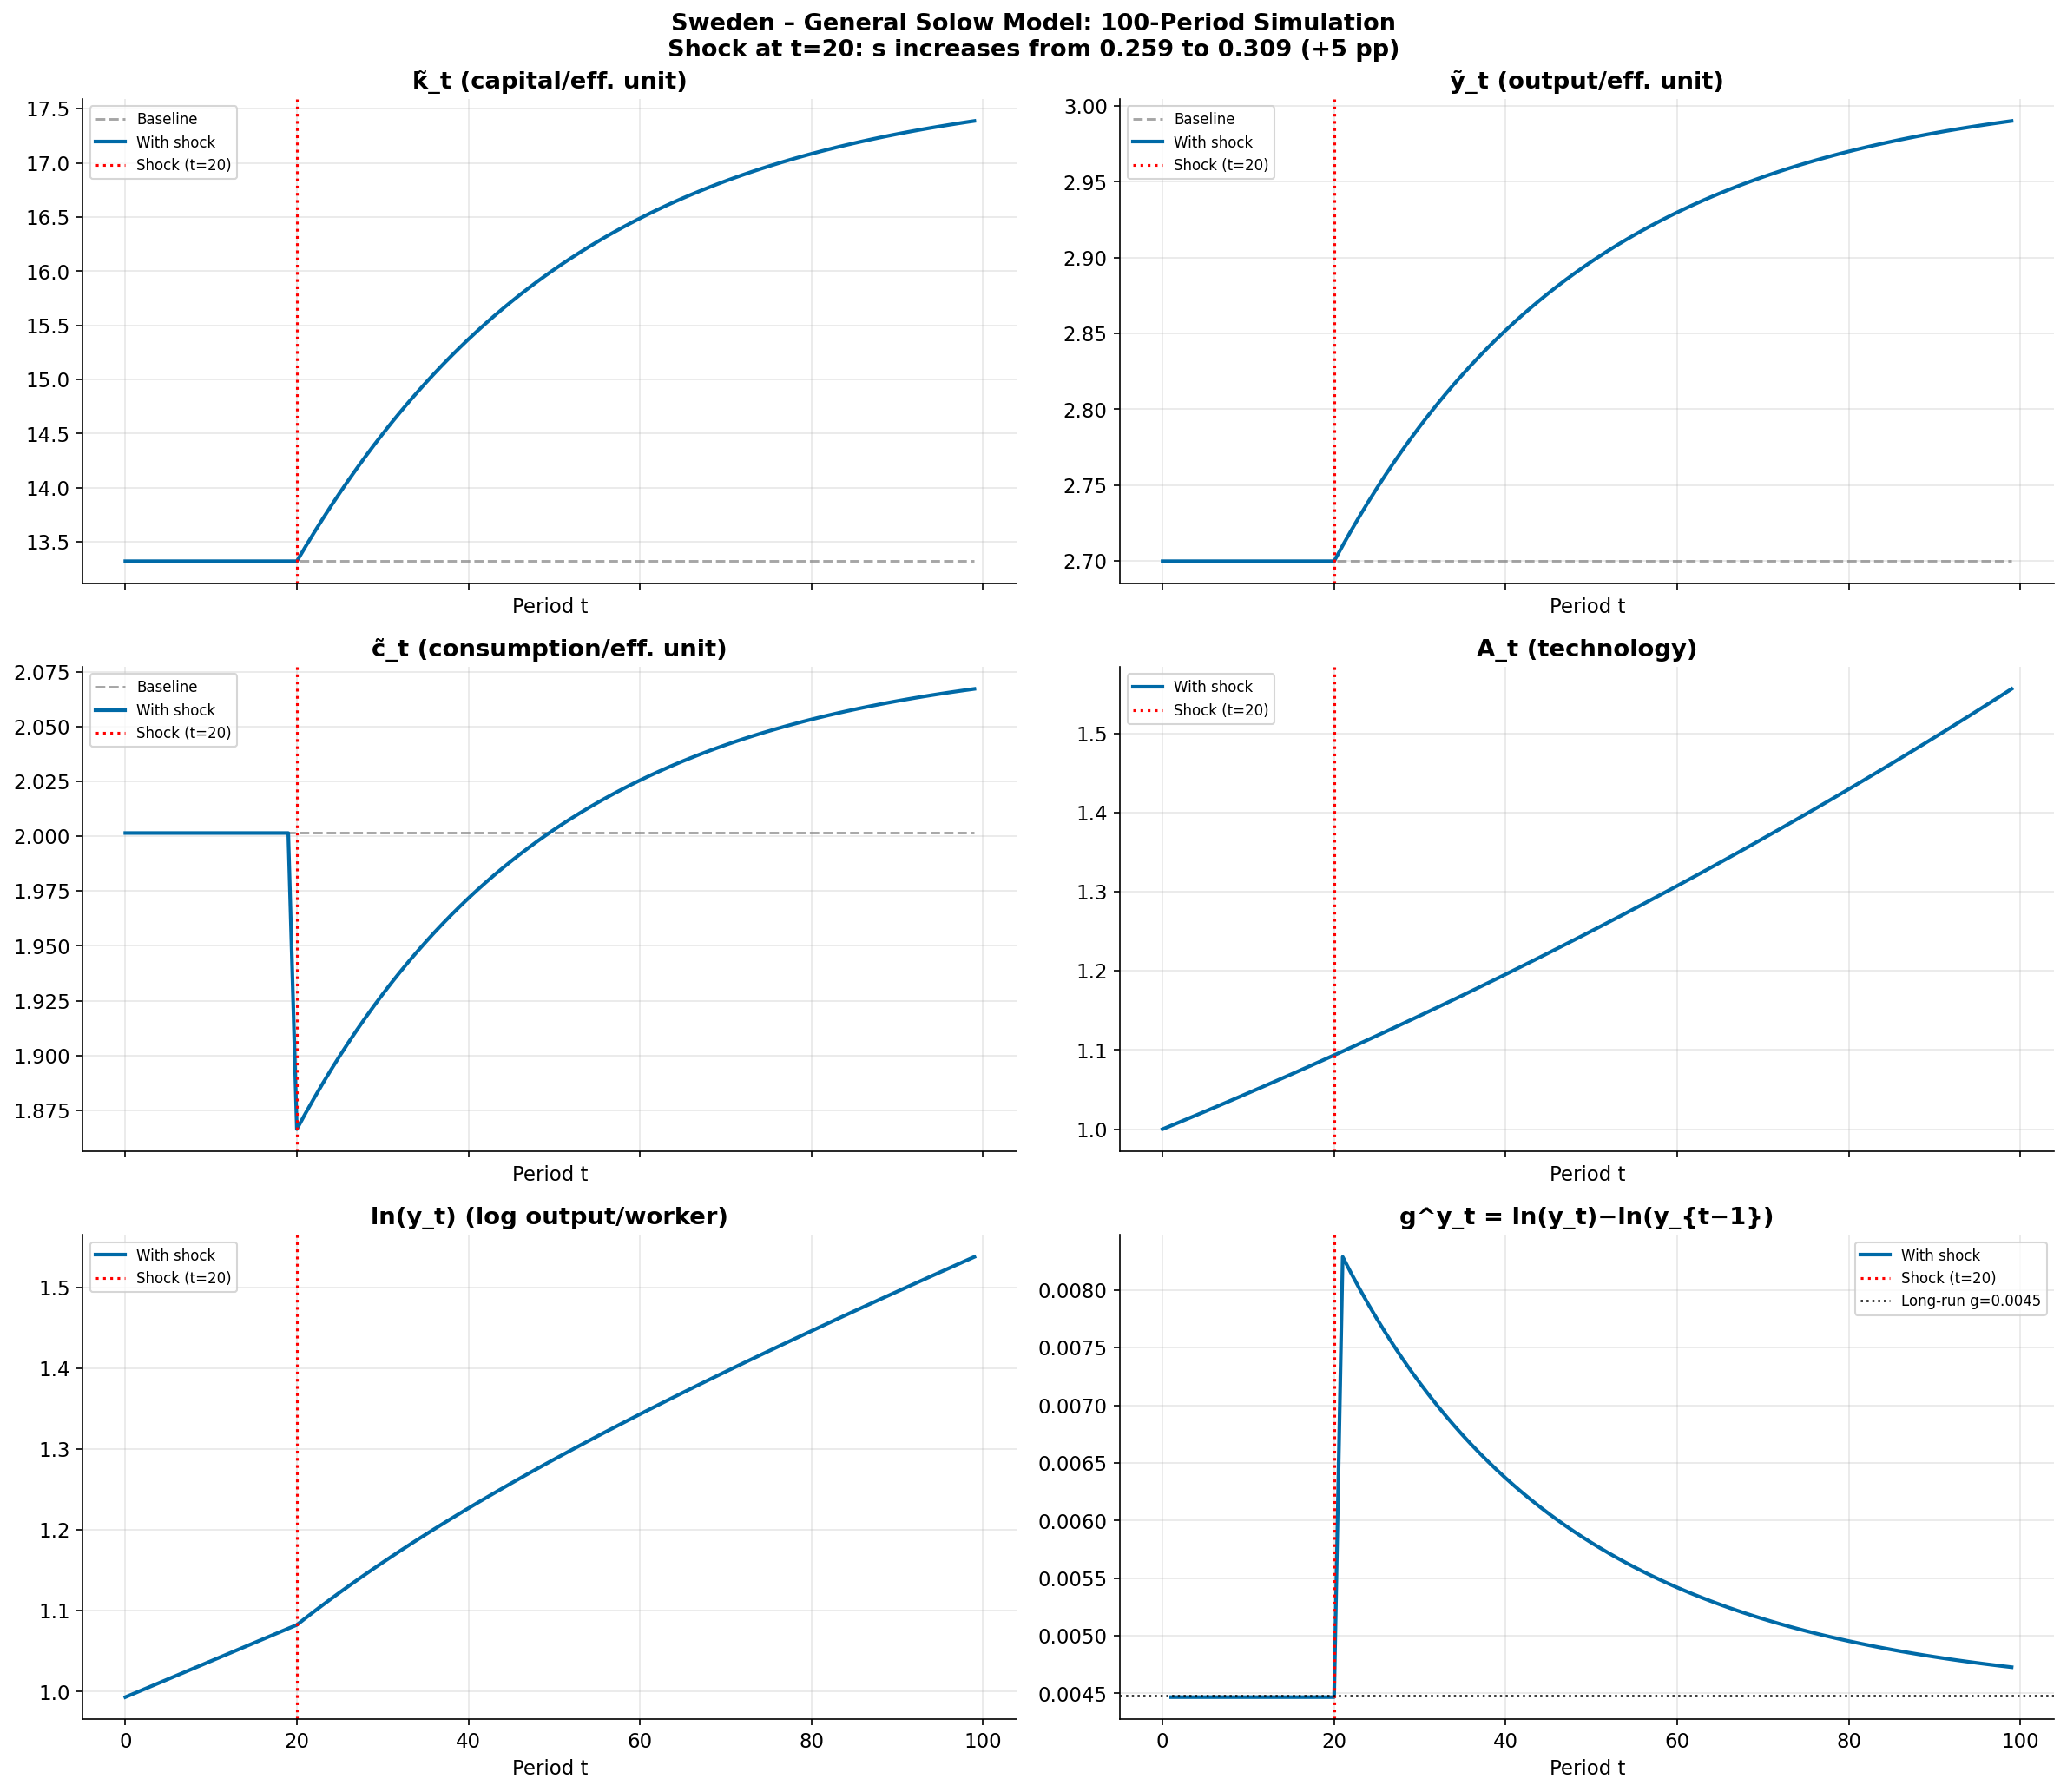
\includegraphics[width=\linewidth]{Sweden/sweden_solow_overview.png}
    \end{column}
    \begin{column}{0.39\textwidth}
      \vspace{0.3cm}
      \small
      \begin{tabular}{@{}Lr@{}}
        \toprule
        \textbf{Parameter} & \textbf{Value} \\
        \midrule
        $\alpha$ & 0.384 \\
        $s$      & 0.259 \\
        $\delta$ & 0.040 \\
        $n$      & 0.008 \\
        $g$      & 0.004 \\
        \midrule
        $\tilde{k}^*$ & 13.32 \\
        $\tilde{y}^*$ & 2.70 \\
        \bottomrule
      \end{tabular}
      \vspace{0.4cm}
      \begin{itemize}\setlength\itemsep{3pt}
        \item $s<\alpha$: below Golden Rule
        \item Savings $\uparrow\Rightarrow\tilde{c}^*\uparrow$ (welfare gain)
        \item Highest TFP growth of three countries
      \end{itemize}
    \end{column}
  \end{columns}
\end{frame}

% ============================================================
%  PART 4 – CROSS-COUNTRY COMPARISON
% ============================================================
\sectionslide{navydark}{Cross-Country Comparison}{Denmark · Norway · Sweden}

% ── Comp 1: GDP & Growth ────────────────────────────────────
\begin{frame}{Comparison – GDP per Capita \& Growth}
  \framesubtitle{Common sample 1993 Q1 – 2024 Q4}
  \begin{columns}[T]
    \begin{column}{0.50\textwidth}
      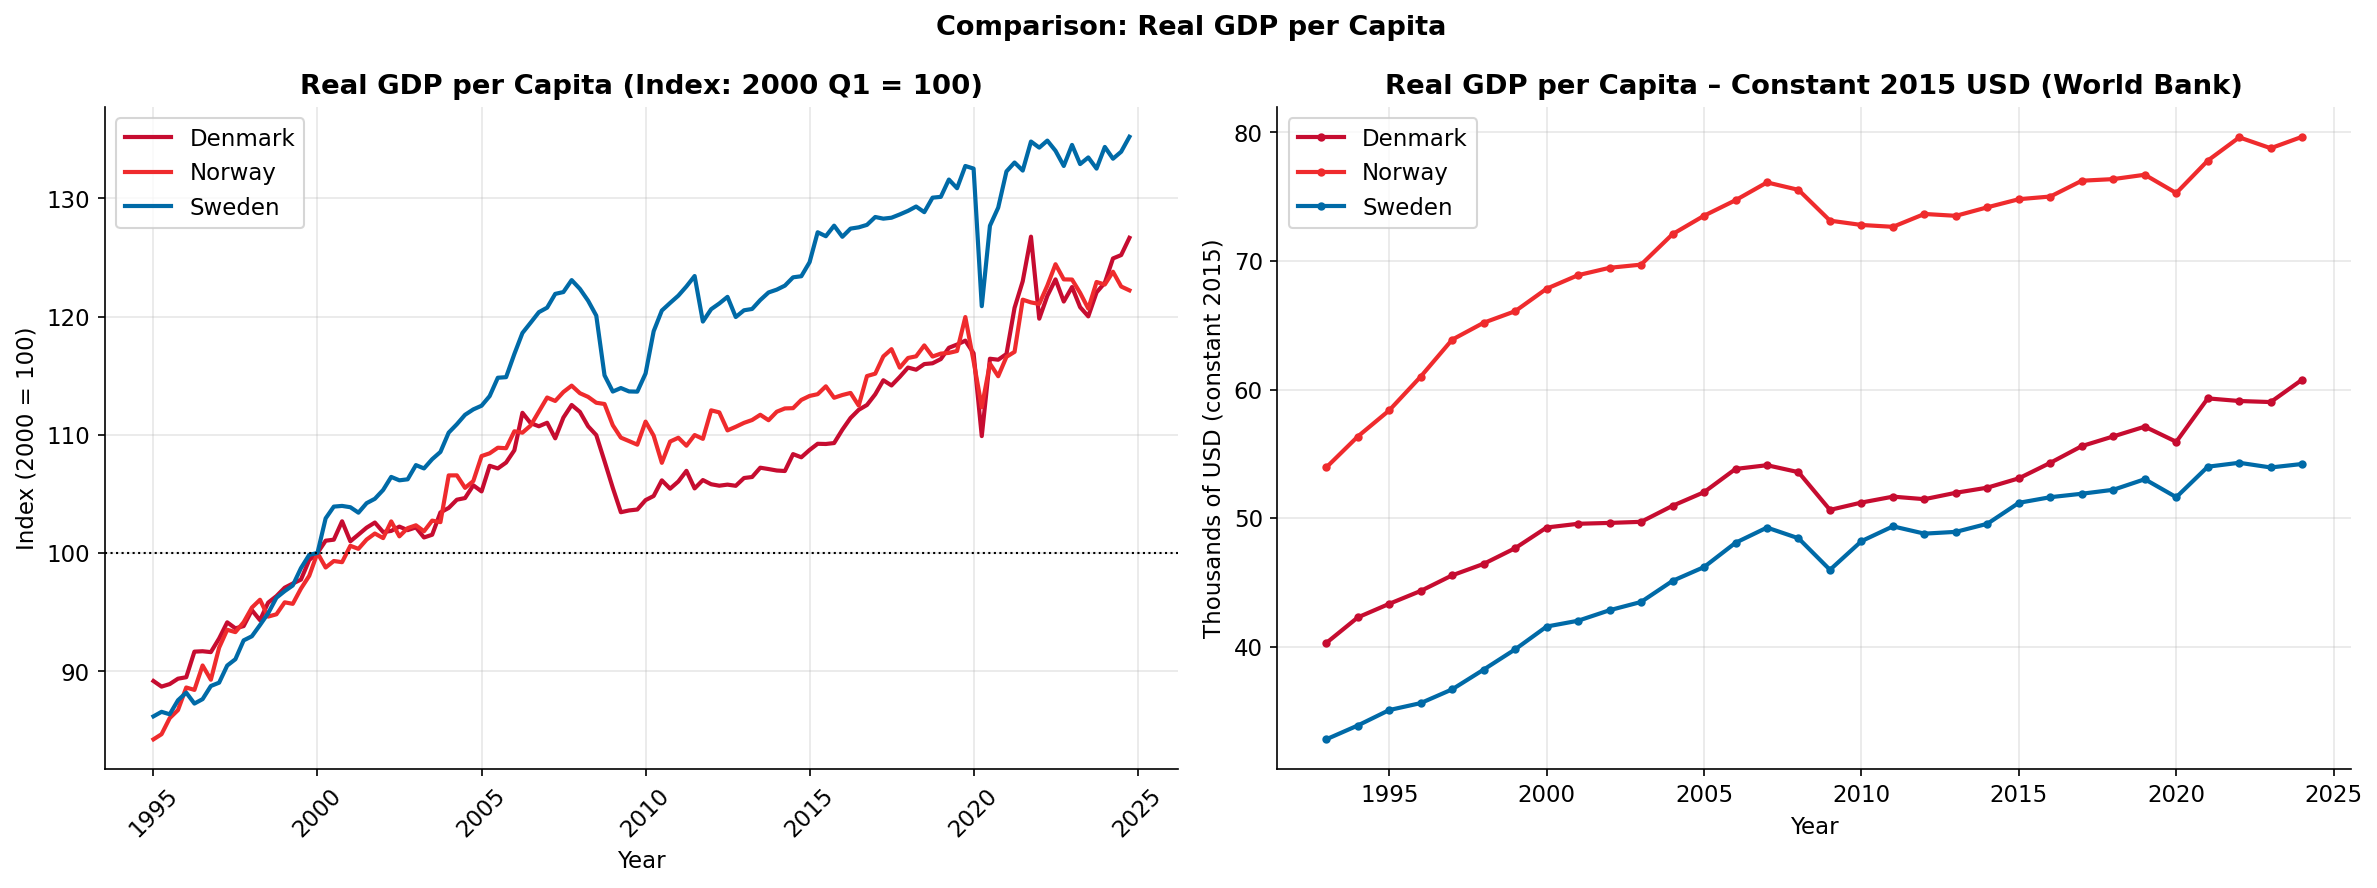
\includegraphics[width=\linewidth]{Part3_Comparison/comparison_gdp_pc.png}
    \end{column}
    \begin{column}{0.47\textwidth}
      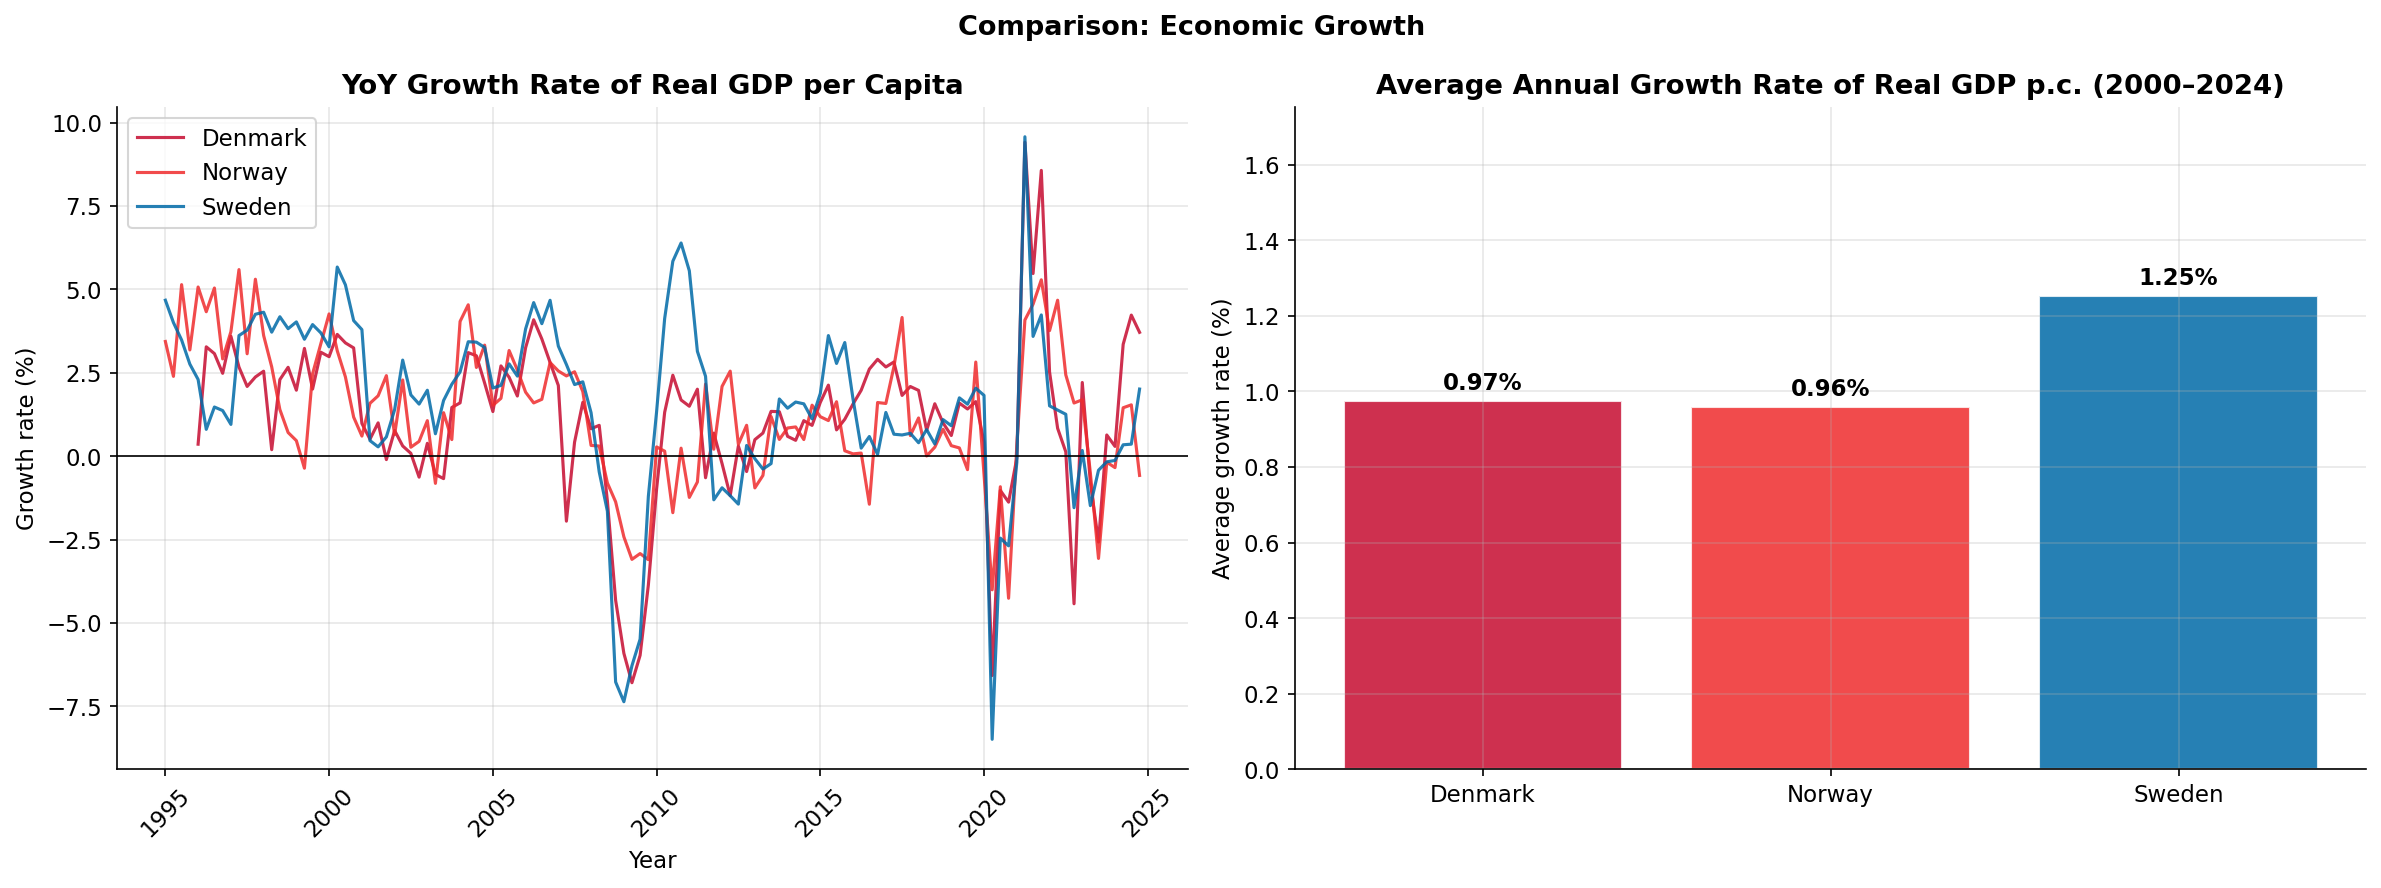
\includegraphics[width=\linewidth]{Part3_Comparison/comparison_growth.png}
    \end{column}
  \end{columns}
  \vspace{0.1cm}
  \small
  \begin{itemize}\setlength\itemsep{2pt}
    \item Norway highest level — oil wealth premium
    \item Sweden fastest trend growth ($\approx1.25\%$); Denmark \& Norway $\approx1.0\%$
    \item All three show synchronised GFC 2008–09 and COVID 2020 dips
  \end{itemize}
\end{frame}

% ── Comp 2: Unemployment & Inflation ────────────────────────
\begin{frame}{Comparison – Labour Market \& Inflation}
  \begin{columns}[T]
    \begin{column}{0.50\textwidth}
      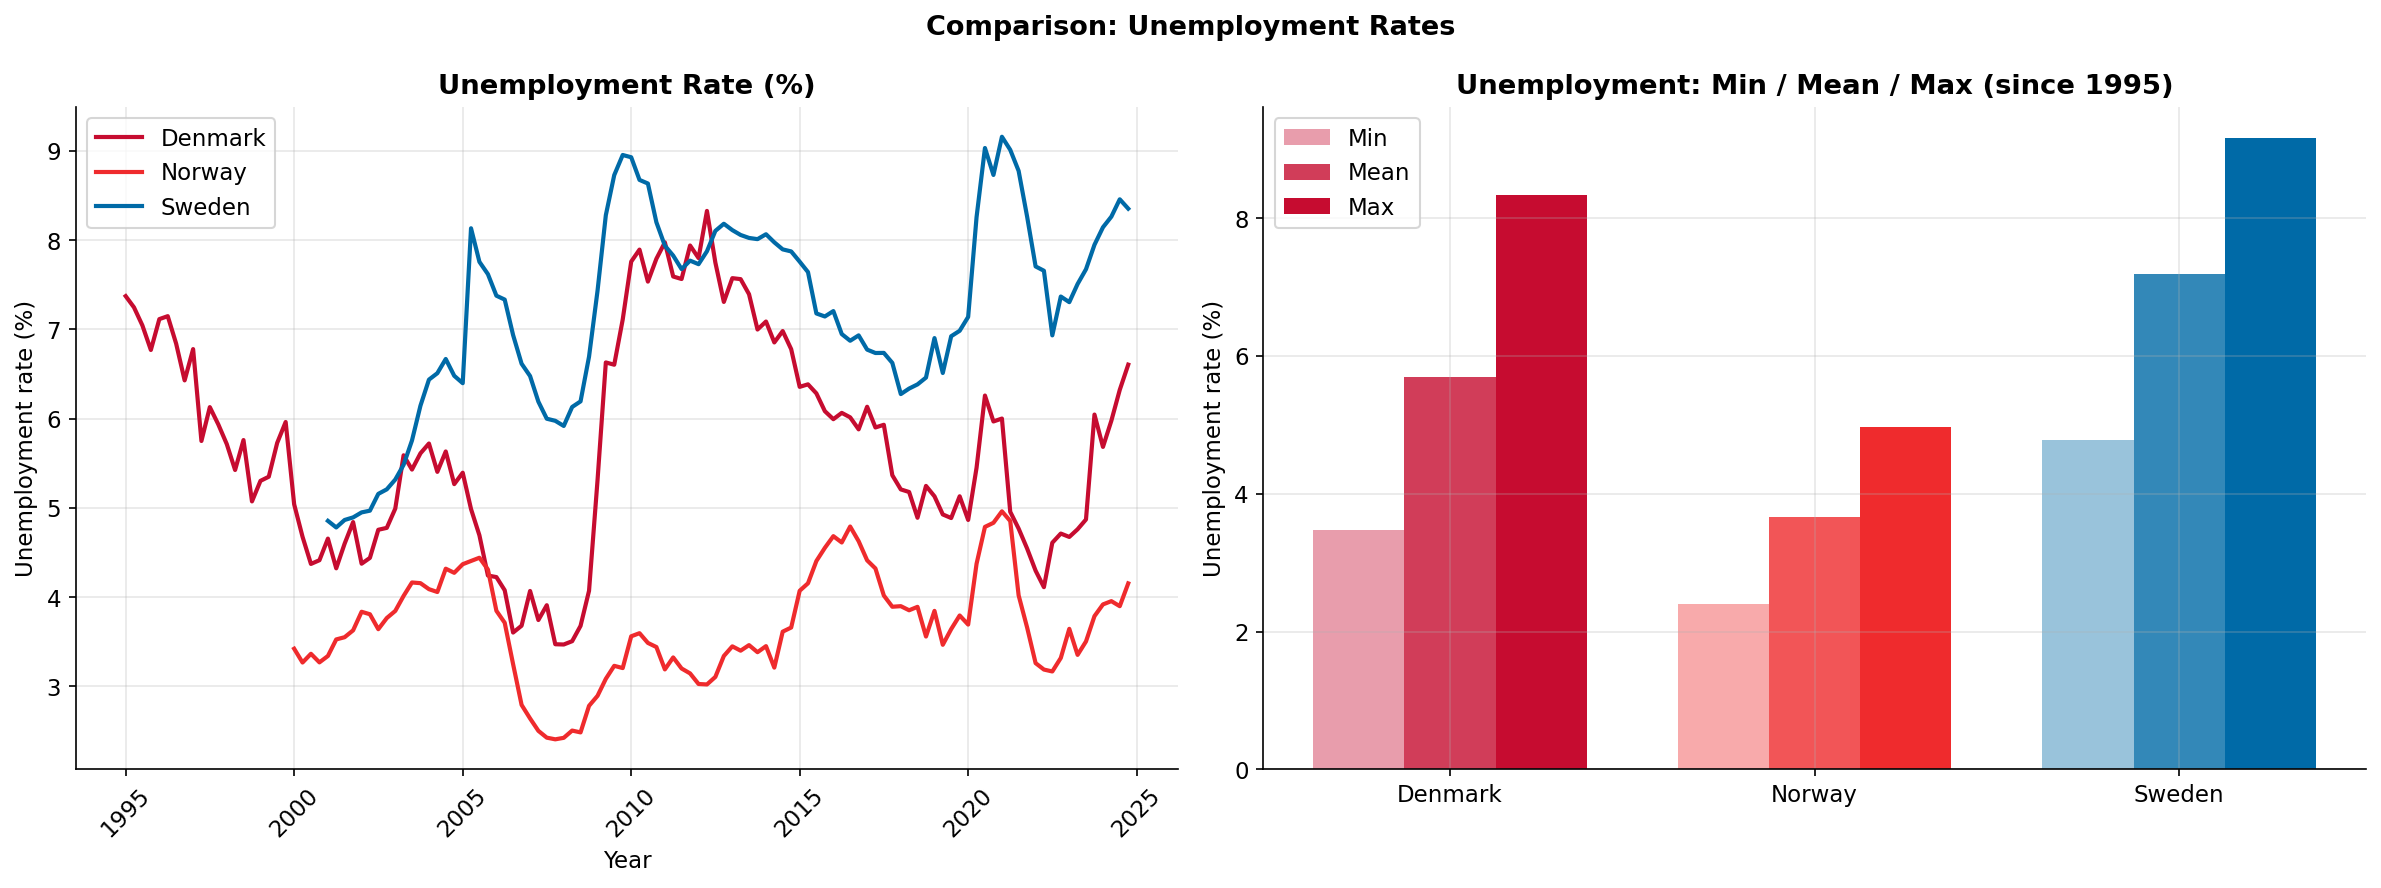
\includegraphics[width=\linewidth]{Part3_Comparison/comparison_unemployment.png}
    \end{column}
    \begin{column}{0.47\textwidth}
      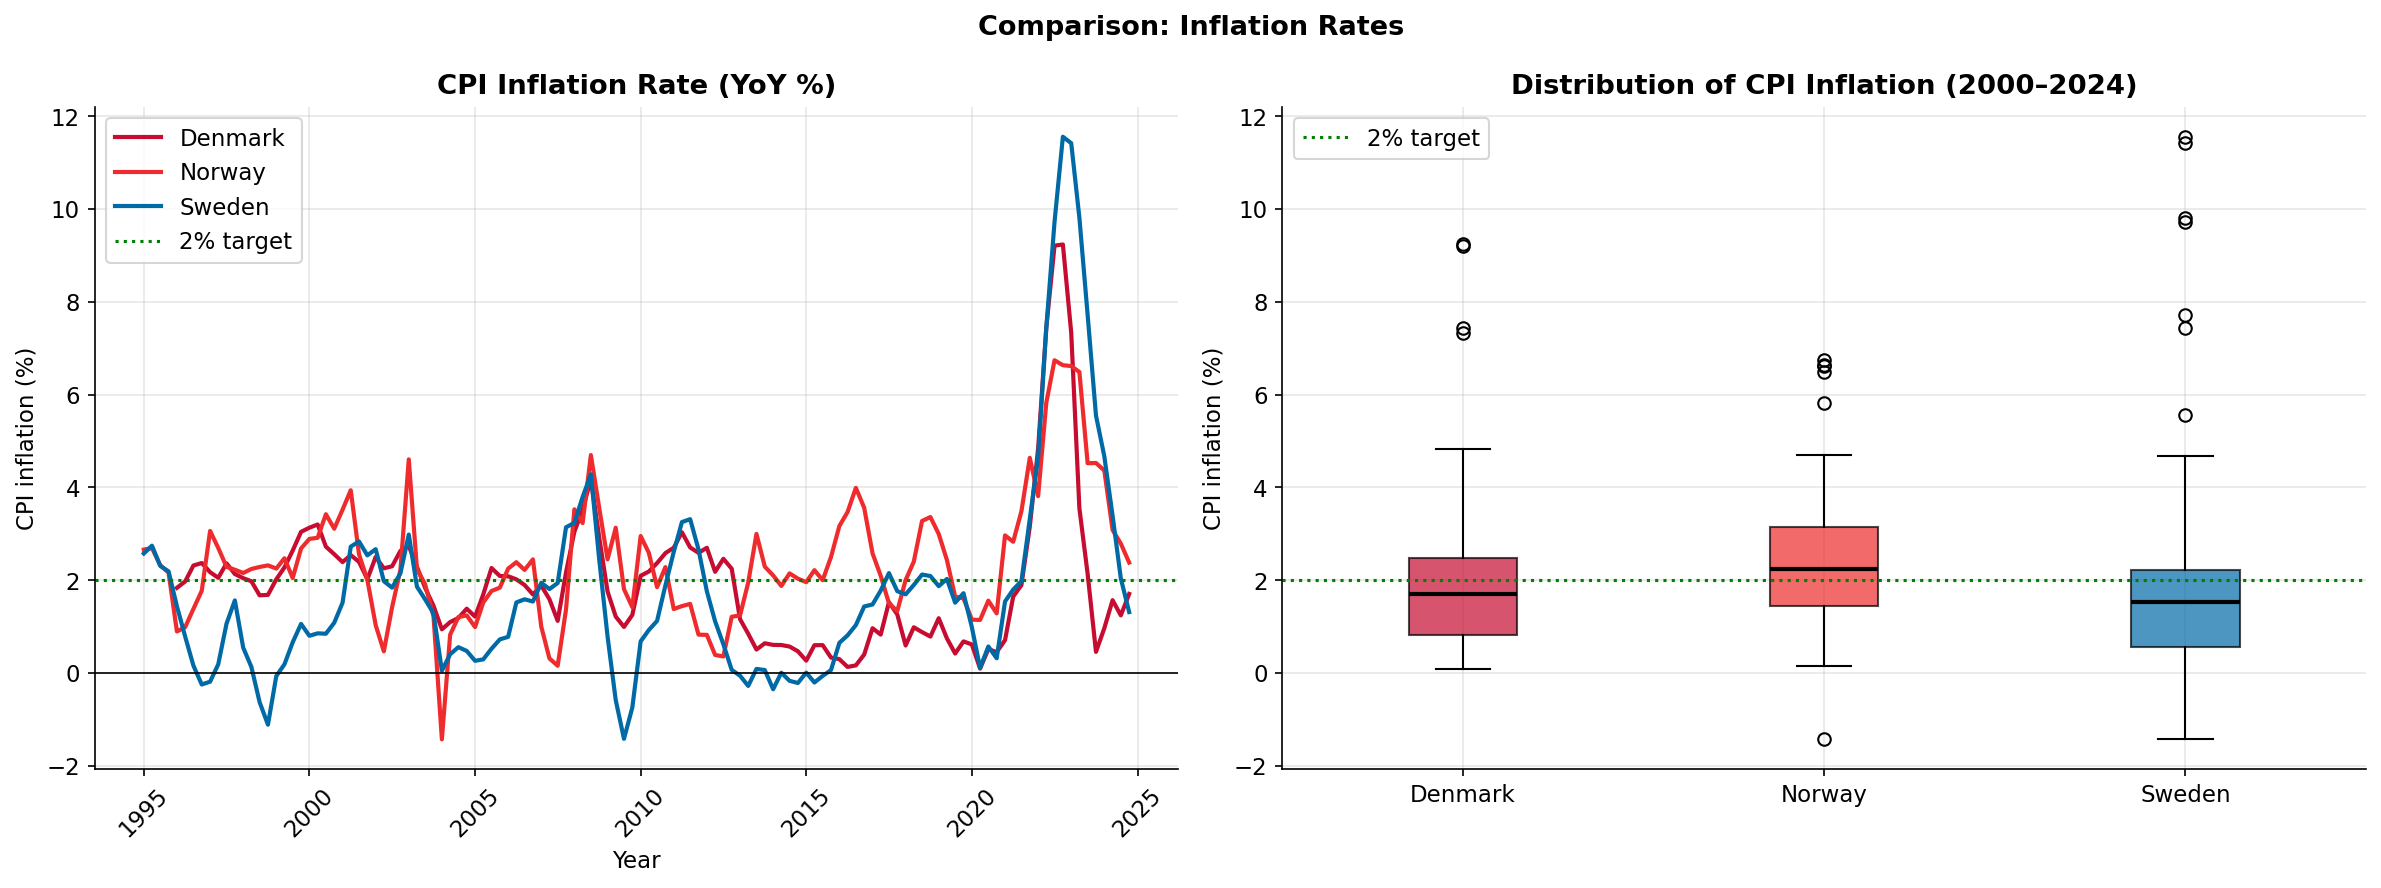
\includegraphics[width=\linewidth]{Part3_Comparison/comparison_inflation.png}
    \end{column}
  \end{columns}
  \vspace{0.1cm}
  \small
  \begin{itemize}\setlength\itemsep{2pt}
    \item Norway lowest unemployment ($\approx3.7\%$); Sweden highest ($\approx6\%$) — ERM legacy
    \item Inflation broadly converged since 2000; post-2021 spike common to all three
    \item Norway oil fund dampens domestic demand swings; Sweden more exposed
  \end{itemize}
\end{frame}

% ── Comp 3: Solow Parameters ────────────────────────────────
\begin{frame}{Comparison – Solow Model}
  \framesubtitle{Cross-country Solow comparison: parameters \& steady states}
  \begin{columns}[T]
    \begin{column}{0.50\textwidth}
      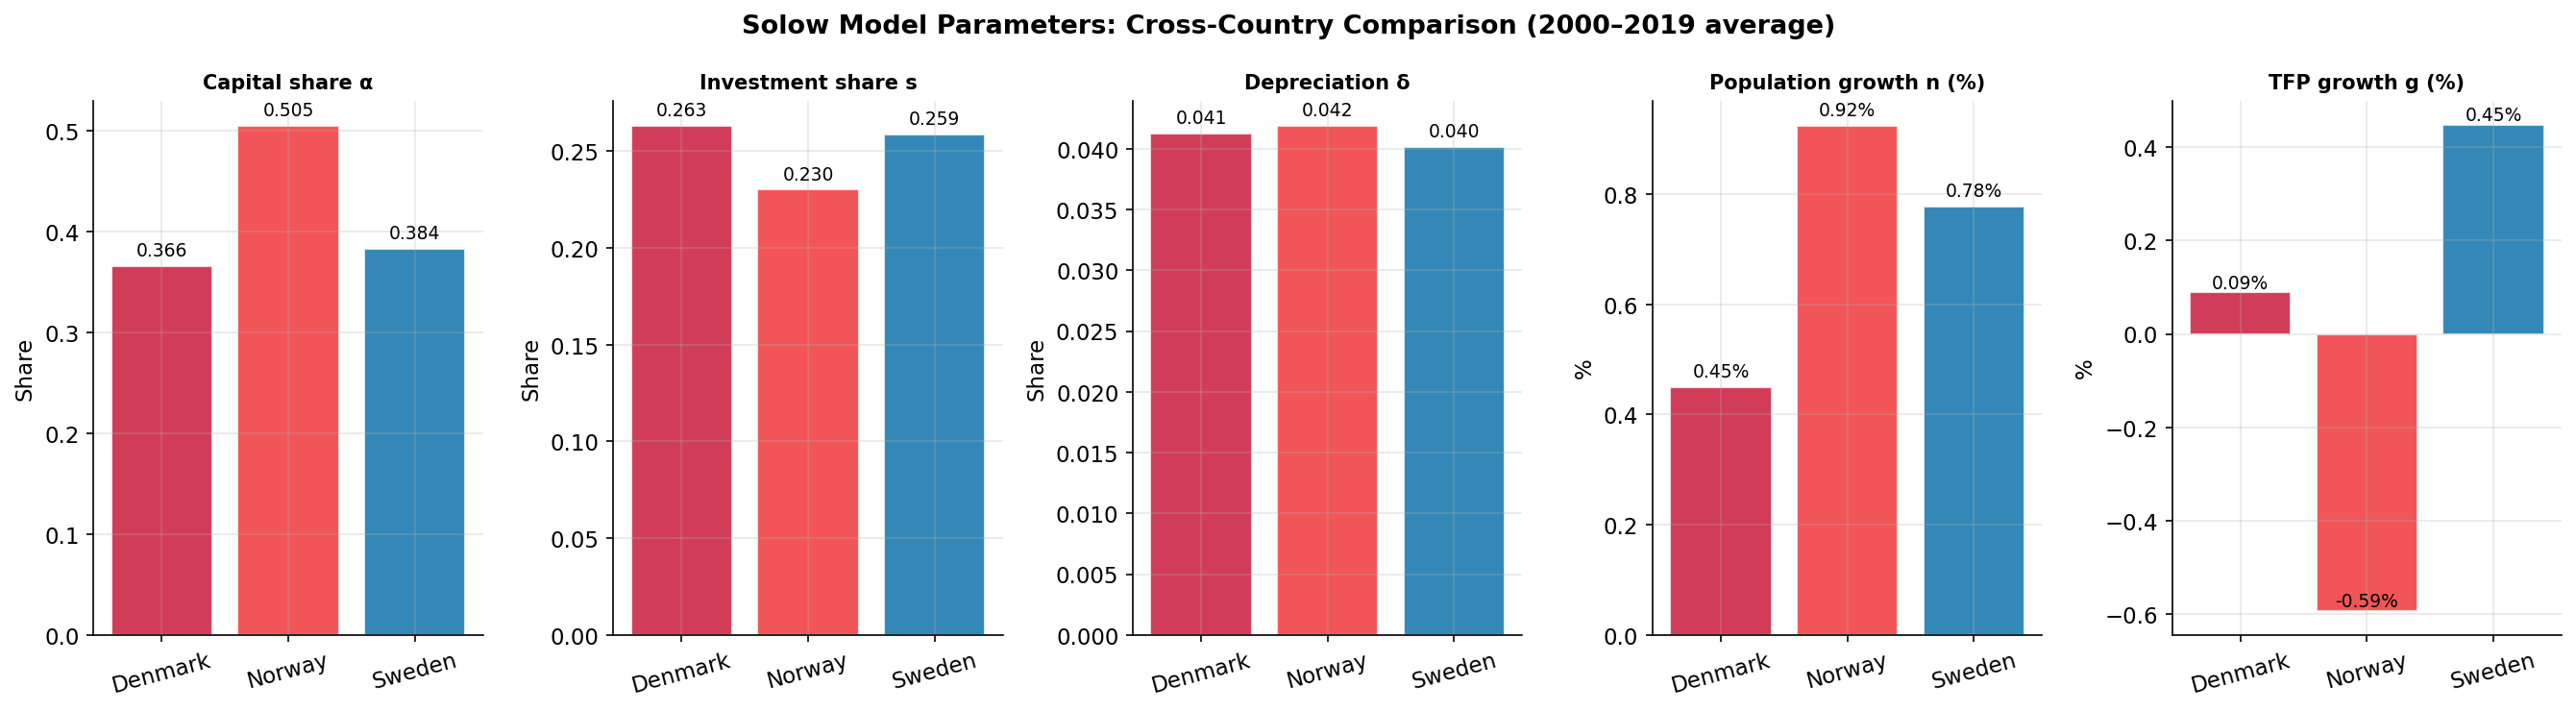
\includegraphics[width=\linewidth]{Part3_Comparison/comparison_solow_params.png}
    \end{column}
    \begin{column}{0.47\textwidth}
      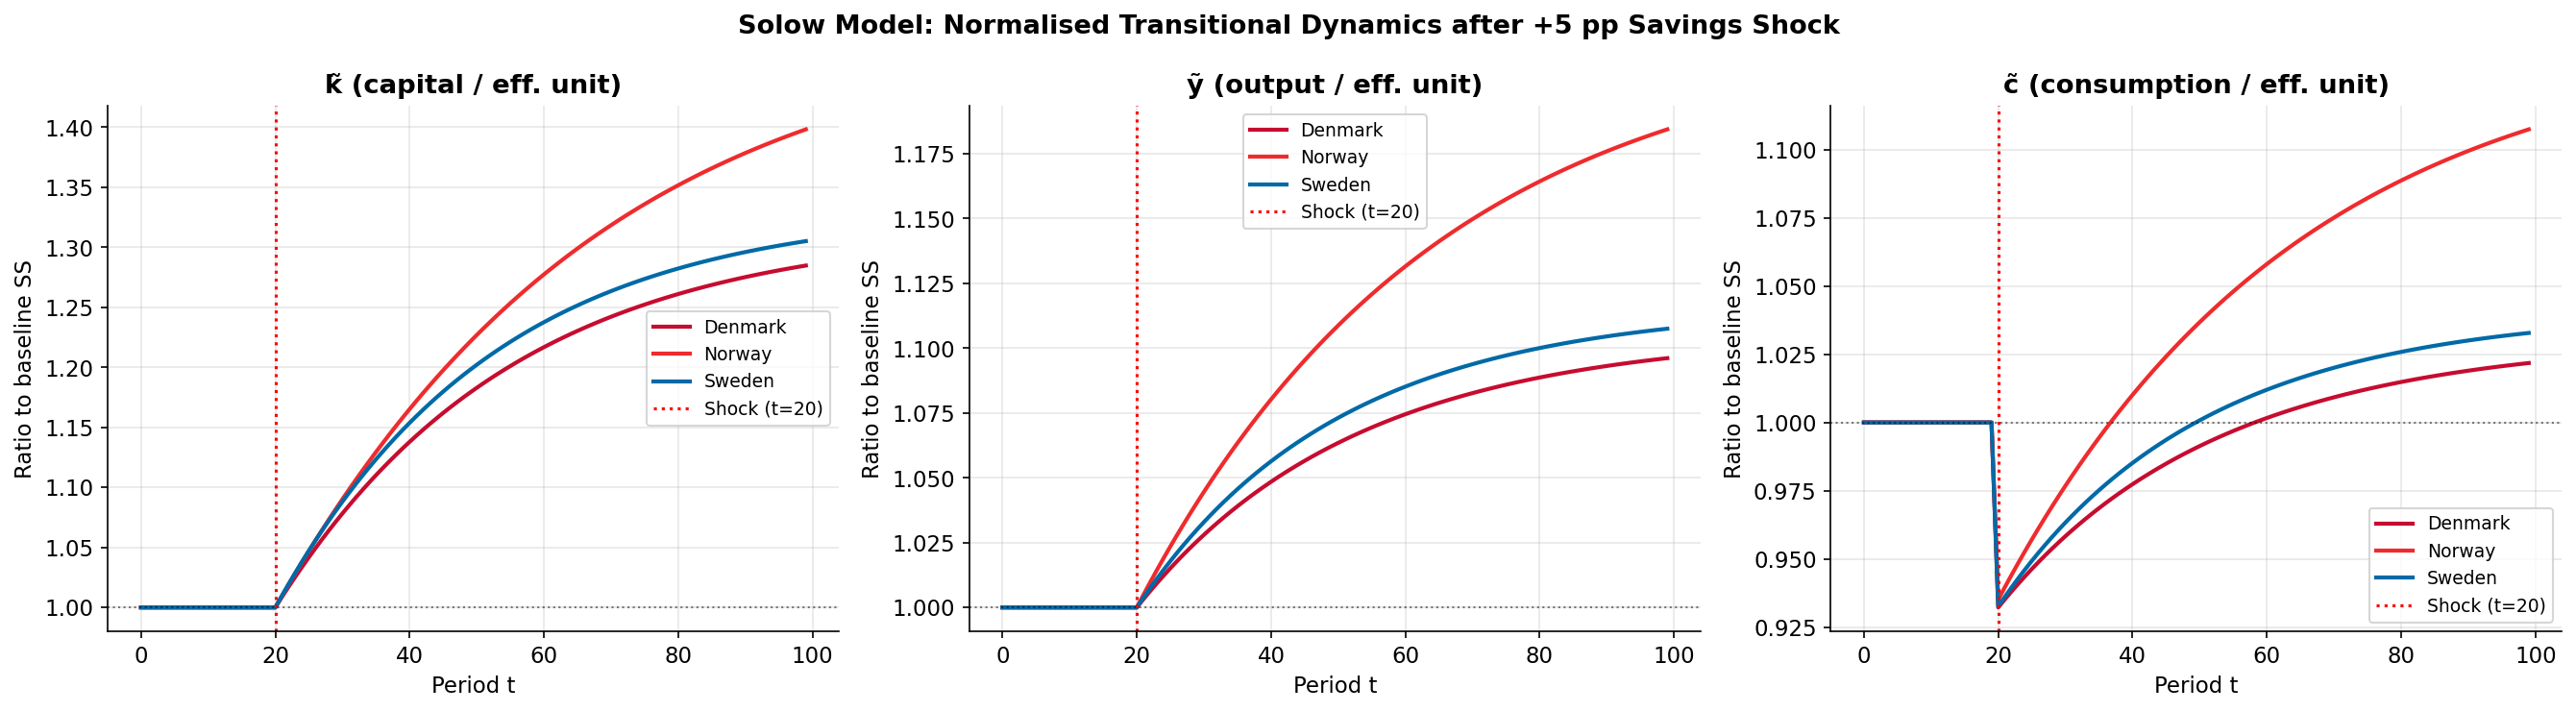
\includegraphics[width=\linewidth]{Part3_Comparison/comparison_solow_tilde.png}
    \end{column}
  \end{columns}
  \vspace{0.1cm}
  \small
  \begin{itemize}\setlength\itemsep{2pt}
    \item Norway outlier: $\alpha=0.505$, $g<0$ — oil distorts both capital share and TFP
    \item Denmark \& Sweden: similar $\alpha\approx0.37$, $g>0$, both below Golden Rule
    \item All three: $s<\alpha$ $\Rightarrow$ savings increase raises steady-state consumption
  \end{itemize}
\end{frame}

\end{document}
